\documentclass[12pt,a4paper,oneside]{report}

% ===== FONT =====
\usepackage{iftex}
\ifPDFTeX
\PackageError{Report}{Compile with XeLaTeX}{Use xelatex}
\fi
\usepackage{fontspec}
\setmainfont{Times New Roman}

% ===== PAGE =====
\usepackage[a4paper,left=3cm,right=2cm,top=2cm,bottom=2cm]{geometry}
\usepackage{setspace}
\setstretch{1.15}

% ===== PACKAGES =====
\usepackage{graphicx}
\usepackage{amsmath}
\usepackage{booktabs}
\usepackage{longtable}
\usepackage{tabularx}
\usepackage{array}
\usepackage{multirow}
\usepackage{float}
\usepackage{hyperref}
\usepackage{caption}
\usepackage{titlesec}
\usepackage{fancyhdr}
\usepackage{tocloft}
\usepackage{newfloat}
\usepackage{enumitem}
\usepackage{etoolbox}
\usepackage{ragged2e}

\hypersetup{
  colorlinks=true,
  linkcolor=black,
  citecolor=black,
  urlcolor=black,
  pdftitle={Jan-Sunwai AI Final Project Report},
  pdfauthor={Project Team},
  pdfsubject={Civic Grievance Redressal Platform},
  pdfkeywords={FastAPI, React, MongoDB, Ollama, Civic AI},
  bookmarksnumbered=true,
  breaklinks=true
}

% ===== SPACING FIX =====
\setlength{\parindent}{0pt}
\setlength{\parskip}{3pt}
\flushbottom

% ===== LIST AND TABLE FORMATTING =====
\setcounter{secnumdepth}{3}
\setcounter{tocdepth}{3}
\setlength{\headheight}{14.5pt}
\setlength{\emergencystretch}{2em}
\setlength{\tabcolsep}{4pt}
\setlength{\extrarowheight}{2pt}
\renewcommand{\arraystretch}{1.2}
\renewcommand{\tabularxcolumn}[1]{>{\RaggedRight\arraybackslash}p{#1}}
\setlist[itemize,1]{label=\textbullet,leftmargin=2.0em,labelsep=0.6em,itemsep=0.35em,topsep=0.35em,parsep=0pt,partopsep=0pt}
\setlist[itemize,2]{label=\textendash,leftmargin=2.2em,labelsep=0.5em,itemsep=0.25em,topsep=0.25em,parsep=0pt,partopsep=0pt}
\setlist[enumerate,1]{label=\arabic*.,leftmargin=2.2em,labelsep=0.6em,itemsep=0.35em,topsep=0.35em,parsep=0pt,partopsep=0pt}
\setlist[enumerate,2]{label=\alph{enumii}.,leftmargin=2.5em,labelsep=0.6em,itemsep=0.25em,topsep=0.25em,parsep=0pt,partopsep=0pt}
\setlist[enumerate,3]{label=\roman{enumiii}.,leftmargin=2.8em,labelsep=0.6em,itemsep=0.2em,topsep=0.2em,parsep=0pt,partopsep=0pt}
\captionsetup{position=bottom,skip=6pt}
\captionsetup[figure]{position=bottom,skip=6pt}
\captionsetup[table]{position=top,skip=6pt}
\captionsetup[longtable]{position=top,skip=6pt}

\AtBeginDocument{\justifying}
\fussy

% ===== HEADINGS =====
\titleformat{\chapter}
{\bfseries\fontsize{16}{19}\selectfont\centering}
{\chaptername\ \thechapter:}{0.5em}{}

\titleformat{\section}
{\bfseries\fontsize{14}{17}\selectfont}
{\thesection}{0.5em}{}

\titleformat{\subsection}
{\bfseries\fontsize{13}{16}\selectfont}
{\thesubsection}{0.5em}{}

\titleformat{\subsubsection}
{\bfseries\fontsize{12}{14}\selectfont}
{\thesubsubsection}{0.5em}{}

% ===== PAGE NUMBER =====
\pagestyle{fancy}
\fancyhf{}
\fancyfoot[C]{\thepage}
\renewcommand{\headrulewidth}{0pt}

\fancypagestyle{plain}{%
  \fancyhf{}
  \fancyfoot[C]{\thepage}
  \renewcommand{\headrulewidth}{0pt}
  \renewcommand{\footrulewidth}{0pt}
}

\newcommand{\setromanfooterstyles}{%
  \pagestyle{plain}
}

\newcommand{\setarabicfooterstyles}{%
  \pagestyle{fancy}
}

% ===== TOC STYLE =====
\renewcommand{\cftchappresnum}{Chapter\ }
\renewcommand{\cftchapaftersnum}{: }
\setlength{\cftchapnumwidth}{6em}

\setlength{\cftchapindent}{0em}
\setlength{\cftsecindent}{1.5em}
\setlength{\cftsubsecindent}{3em}

\renewcommand{\cftdotsep}{1}

% ===== CENTERED CONTENTS TITLE =====
\makeatletter
\renewcommand{\tableofcontents}{
  \clearpage
  \phantomsection
  {\centering\bfseries\fontsize{16}{19}\selectfont Contents\par}
  \vspace{1em}
  \@starttoc{toc}
}
\makeatother

% ===== LIST NAMES =====
\renewcommand{\listfigurename}{List of Figures}
\renewcommand{\listtablename}{List of Tables}

% ===== CUSTOM COMMANDS =====
\newcommand{\placeholderfigure}[2]{
\begin{figure}[H]
\centering
\fbox{\begin{minipage}[c][2.6in][c]{0.85\textwidth}
\centering
\textbf{#1}\\[0.6em]
\small #2
\end{minipage}}
\caption{#1}
\end{figure}
}

\newcommand{\screenshotcard}[5][]{%
\begin{screenshot}[H]
\centering
\IfFileExists{#4}{%
  \includegraphics[width=0.96\textwidth,height=0.28\textheight,keepaspectratio]{#4}%
}{%
  \fbox{\begin{minipage}[c][0.26\textheight][c]{0.90\textwidth}
  \centering
  \textbf{Screenshot Placeholder}\\[0.5em]
  \small Missing file: #4
  \end{minipage}}%
}
\ifstrempty{#1}{%
  \caption{#5}%
}{%
  \caption[#1]{#5}%
}
\label{#3}
\end{screenshot}
}

% ===== SCREENSHOTS =====
\DeclareFloatingEnvironment[
    fileext=los,
    listname={List of Screenshots},
    name=Screenshot
]{screenshot}

\renewcommand{\thescreenshot}{\thechapter.\arabic{screenshot}}

% ===== DOCUMENT START =====
\begin{document}

\pagenumbering{roman}
\setromanfooterstyles

% ===== FRONT MATTER =====
% Minimal inner title page placeholder to allow compilation
\begin{titlepage}
  \centering
  {\LARGE Jan-Sunwai AI\\[1ex]}
  {\large Technical Report\\[3ex]}
  {\large April 2026\\[4ex]}
  \vfill
  \begin{flushright}
    \large Prepared by the Jan-Sunwai Team\\[1ex]
  \end{flushright}
\end{titlepage}
\begin{titlepage}
\centering
\vspace*{1.2cm}
{\Large \textbf{Final Year Project Report}}\\[0.6cm]
{\LARGE \textbf{Jan-Sunwai AI}}\\[0.3cm]
{\large Automated Visual Classification, Routing, and Lifecycle Tracking\\for Civic Grievances}\\[1.2cm]

\includegraphics[width=0.23\textwidth]{gui_wireframe.png}\\[1.0cm]

\begin{tabular}{p{0.35\textwidth}p{0.55\textwidth}}
Project Domain: & Civic Technology and Grievance Redressal \\
Technology Stack: & React, FastAPI, MongoDB, Ollama, Docker \\
Academic Session: & 2025--2026 \\
Project Duration: & 28 January 2026 -- 27 May 2026 \\
Submission Type: & Major Project Final Report \\
\end{tabular}

\vfill

\begin{tabular}{p{0.35\textwidth}p{0.55\textwidth}}
Submitted By: & \textit{Project Team} \\
Guided By: & \textit{Project Supervisor} \\
Department: & \textit{Computer Science / Information Technology} \\
Institute: & \textit{Institution Name} \\
\end{tabular}

\vspace*{1.0cm}
\end{titlepage}

\newpage
% Minimal inner title page placeholder to allow compilation
\begin{titlepage}
  \centering
  {\LARGE Jan-Sunwai AI\\[1ex]}
  {\large Technical Report\\[3ex]}
  {\large April 2026\\[4ex]}
  \vfill
  \begin{flushright}
    \large Prepared by the Jan-Sunwai Team\\[1ex]
  \end{flushright}
\end{titlepage}
\begin{titlepage}
\centering
\vspace*{1.2cm}
{\Large \textbf{Final Year Project Report}}\\[0.6cm]
{\LARGE \textbf{Jan-Sunwai AI}}\\[0.3cm]
{\large Automated Visual Classification, Routing, and Lifecycle Tracking\\for Civic Grievances}\\[1.2cm]

\includegraphics[width=0.23\textwidth]{gui_wireframe.png}\\[1.0cm]

\begin{tabular}{p{0.35\textwidth}p{0.55\textwidth}}
Project Domain: & Civic Technology and Grievance Redressal \\
Technology Stack: & React, FastAPI, MongoDB, Ollama, Docker \\
Academic Session: & 2025--2026 \\
Project Duration: & 28 January 2026 -- 27 May 2026 \\
Submission Type: & Major Project Final Report \\
\end{tabular}

\vfill

\begin{tabular}{p{0.35\textwidth}p{0.55\textwidth}}
Submitted By: & \textit{Project Team} \\
Guided By: & \textit{Project Supervisor} \\
Department: & \textit{Computer Science / Information Technology} \\
Institute: & \textit{Institution Name} \\
\end{tabular}

\vspace*{1.0cm}
\end{titlepage}

\newpage
\chapter*{Dedication}
\addcontentsline{toc}{chapter}{Dedication}

This project report is dedicated to all mentors, faculty members, and families whose support made this work possible.

\newpage
\chapter*{Student Declaration}
\addcontentsline{toc}{chapter}{Student Declaration}

I hereby declare that this project report titled \textit{Jan-Sunwai AI} is my/our original work carried out under the guidance of the project supervisor, and has not been submitted elsewhere for any other degree or diploma.

\vspace{2cm}
\noindent Name(s) of Student(s): \hrulefill

\vspace{1cm}
\noindent Signature(s): \hrulefill

\vspace{1cm}
\noindent Date: \hrulefill

\newpage
\chapter*{Certificate from Supervisor (MUJ)}
\addcontentsline{toc}{chapter}{Certificate from Supervisor (MUJ)}

This is to certify that the project report titled \textit{Jan-Sunwai AI} has been carried out by the student(s) under my supervision and guidance as partial fulfillment of the degree requirements.

\vspace{2cm}
\noindent Name of Supervisor: \hrulefill

\vspace{1cm}
\noindent Signature: \hrulefill

\vspace{1cm}
\noindent Date: \hrulefill

\newpage
\chapter*{Certificate on Company Letter Head}
\addcontentsline{toc}{chapter}{Certificate on Company Letter Head}

Attach the xerox copy of the company certificate here. The original must be retained by the student.

\newpage
\chapter*{Acknowledgement}
\addcontentsline{toc}{chapter}{Acknowledgement}

We express our sincere gratitude to our project supervisor and the department faculty for their unwavering guidance, technical insights, and continuous encouragement throughout the development of the Jan-Sunwai AI platform. Their constructive feedback was instrumental in shaping the architecture and governance focus of this project.

We also extend our thanks to the open-source communities behind FastAPI, React, MongoDB, and the Ollama ecosystem. The availability of robust, community-driven tools made the local-first execution of this vision-language pipeline a reality. Finally, we would like to thank our peers and all individuals who participated in the user acceptance testing, as their practical insights directly contributed to the system's final accessibility and workflow design.

\newpage
\chapter*{Abstract}
\addcontentsline{toc}{chapter}{Abstract}

Jan-Sunwai AI addresses the critical friction in municipal grievance redressal systems, where citizens struggle to correctly categorize their complaints and authorities lack the triage bandwidth to route them efficiently. This project presents a hybrid AI-assisted platform that combines automated vision-language classification (via Llama 3.2 Vision) with deterministic, role-based governance workflows. The system transforms unstructured image uploads into structured, auditable tasks while preserving human-in-the-loop oversight for edge cases. Implemented with a scalable architecture using React, FastAPI, MongoDB, and Docker, the platform was evaluated under simulated municipal loads. Performance testing validated the approach, achieving an average classification confidence of 0.78 for civic imagery, a low fallback rate of 4.2%, and a sustained API response time of 320ms. The results demonstrate that integrating edge AI into civic infrastructure can significantly reduce administrative triage overhead without sacrificing operational transparency or accountability.
\newpage

% ===== TOC =====
\tableofcontents
\newpage

\addcontentsline{toc}{chapter}{List of Tables}
\listoftables
\newpage

\addcontentsline{toc}{chapter}{List of Figures}
\listoffigures
\newpage

\addcontentsline{toc}{chapter}{List of Screenshots}
\listofscreenshots
\newpage

% ===== MAIN =====
\pagenumbering{arabic}
\setarabicfooterstyles

% !TEX root = ../main.tex
\chapter{Introduction}

Jan-Sunwai AI is an end-to-end civic grievance redressal platform designed to minimize the operational delay between when a citizen submits a complaint and when the relevant department takes action. The system converts an image upload into a structured, auditable complaint flow and forwards the case to accountable municipal actors. To remove the need for citizens to navigate bureaucratic department structures, the platform uses AI to classify and draft complaints while keeping a human-controlled correction route via triage and administrative controls.

The project is a local-first system built to meet practical constraints in the municipal domain, where cloud deployment may be limited due to policy, infrastructure, or privacy concerns. The architecture combines a React frontend, a FastAPI backend, MongoDB for the database, and locally-run Ollama models in a hybrid inference pipeline. This deployment approach allows the platform to operate within the narrow confines of institutional settings without sacrificing modularity for future expansion.

\section{Project Details}
\label{sec:project-details}

Jan-Sunwai AI is a civic grievance management platform modelled on NDMC-style municipal governance operations, developed between 28 January and 27 May 2026. Its primary application domain is civic grievance management and municipal operations, serving citizens, workers, department heads, and administrators. The system is implemented as a local-first, containerised stack that runs independently of managed cloud services.

\section{Purpose}

Traditional grievance mechanisms place a significant cognitive load on the very people they are designed to serve. Submitters are typically required to type detailed textual descriptions, navigate multi-level department dropdown menus, and in many cases physically call an office to have a complaint referred to the appropriate person. Citizens who are unfamiliar with municipal organisational structures routinely complain to the wrong department, triggering inter-departmental transfer cycles that delay field action by three to five working days per misrouting event. In such cases, complaint narratives tend to be incomplete, inconsistently formatted, or factually imprecise, requiring substantial clarification from departmental staff before any field response is possible.

Jan-Sunwai AI was built to break this cycle at the earliest stage. Photographic evidence submitted by a citizen is analysed using a vision-language model to derive a visual summary, a probable departmental category, geospatial metadata, and a formally drafted complaint description. The citizen then reviews and, if necessary, edits this output before submission, ensuring that even a non-technical user can produce a structurally sound, verifiable complaint. Complaints arrive pre-classified with AI-generated rationale attached, allowing supervisory effort to focus on resolution governance rather than intake remediation. Administrative stakeholders are provided with an analytics layer, a public transparency feed, and exportable complaint datasets to support operational management and institutional accountability. The intent of the design is not to replace decisions made by human administrators, but to minimise the repetitive manual effort that currently creates barriers to timely field action.

\section{Scope}

The implemented scope covers intake, classification, routing metadata, assignment, notifications, escalation support, and governance analytics. Specifically, the platform includes:

\begin{itemize}
\item User management and role-aware access control
\item AI image analysis and complaint drafting
\item Complaint lifecycle actions: create, track, update, transfer, escalate, and close
\item Worker assignment controls and department-specific work queues
\item A triage procedure for low-confidence classifications or ambiguous cases
\item Notification chains and password reset mechanisms
\item A public-facing complaint listing and operational analytics (anonymised)
\end{itemize}

Multilingual voice input, direct integration with external municipal ERP systems, and predictive resource planning beyond dashboard analytics are currently outside scope.

\section{Objectives}

\subsection{Intake Friction}

Submission friction was recognised as the primary barrier to complaint quality. The intake workflow was built around a simplified upload-analyse-submit sequence where AI-generated content reduces the volume of manual text entry from the citizen. Drafts can be accepted as-is or edited before submission, preserving citizen autonomy while standardising the structural quality of submitted records.

\subsection{Routing Quality}

Routing quality was approached via a canonical department taxonomy and a deterministic authority-mapping algorithm. In place of relying solely on model classification, the system uses rule-based scoring as a governance boundary to ensure that even when model confidence is low, the assigned department remains within a bounded, valid set of municipal authorities.

\subsection{Operational Traceability}

Operational traceability was embedded at every stage of the complaint lifecycle. Each status transition records the responsible actor's identity, a timestamp, and an accompanying message. This audit trail enables supervisory review, escalation adjudication, and post-resolution accountability assessment.

\subsection{Worker Assignment}

Worker assignment automation was implemented via a service that matches complaints to eligible field workers on the basis of departmental alignment, service-area proximity, and current task load. Administrative staff retain the ability to override automated assignments when the algorithm produces an unsuitable result.

\subsection{Security}

Security was made a first-order requirement rather than a post-development hardening exercise. Cookie-session authentication, input sanitisation on all payloads, MIME-type and magic-number validation on file uploads, and full HTTP security headers were specified in the initial architecture and implemented before the feature set was considered complete.

\subsection{Governance and Analytics}

Public transparency and governance analytics were delivered to satisfy the accountability requirement of civic technology. An anonymised public complaint feed and an administrative analytics dashboard, which includes geospatial heatmaps, allow citizens and oversight bodies to observe aggregate system behaviour without exposing personally identifiable information.

\subsection{Production Deployment}

Production deployment readiness was treated as an explicit deliverable. Docker Compose orchestration, environment variable templates, runbooks, and a verification procedure were produced to ensure institutional handover does not require the receiving organisation to reconstruct deployment knowledge from source code.

\section{Technology Stack Used}

The system is built on a five-layer stack. The \textbf{frontend} uses React and Vite for role-based dashboards and authentication-aware routing. The \textbf{backend API} is built with FastAPI and Python, handling REST endpoints, validation, and middleware. \textbf{MongoDB} provides document storage for users, complaints, notifications, and reset tokens. \textbf{Ollama} models serve as the local AI runtime for vision extraction, reasoning, and draft generation. \textbf{Docker Compose} orchestrates the full stack for reproducible dev and production deployment. Testing is handled by pytest~\cite{pytest_docs}, httpx, and locust, covering unit, integration, security, resilience, and load scenarios.

\section{Problem Context and Motivation}

The scale of India's national grievance infrastructure makes routing accuracy an operational issue rather than a clerical one. The CPGRAMS Annual Report 2022-23 records more than 19 lakh grievances at the national level during that financial year~\cite{cpgrams_report}. Work on urban local body portals shows a consistent delay pattern: when a complaint is sent to the wrong department, it typically takes three to five additional working days to reach the correct office because each transfer restarts the review cycle~\cite{world_bank_digital_governance}. That delay matters most in services such as Civil Works or Vector-Borne Disease Control, where the difference between an hour and a day can change the outcome of field response.

Jan-Sunwai AI addresses this bottleneck at the intake stage by combining vision-language classification with a deterministic routing engine, thereby reducing the cognitive burden placed on citizens who do not possess institutional knowledge of departmental jurisdiction. Governance authority over ambiguous cases remains with human administrators, who adjudicate low-confidence classifications through a dedicated triage queue. The balance between AI-assisted automation and human institutional control constitutes the defining architectural principle of the system.

\section{Literature Review}

The literature review for this project focuses on civic-tech complaint systems, AI-assisted classification workflows, and governance requirements such as traceability and explainability. Rather than treating model accuracy as the only success metric, the review emphasizes operational outcomes such as routing correctness, audit readiness, and response-time reliability in public-sector environments. The selected architectural direction in Jan-Sunwai AI was derived from this practical lens~\cite{un_e_gov, world_bank_digital_governance, fielding_rest, hitl_ai}.

\subsection{Digital Governance and Complaint Systems}

Digital grievance platforms are a recognized mechanism for increasing civic participation and service responsiveness. At the national level, frameworks like India's Centralised Public Grievance Redress and Monitoring System (CPGRAMS) have set precedents for digital complaint routing across ministerial departments. Similarly, under the Smart Cities Mission~\cite{smart_cities_mission}, municipal bodies and the National Informatics Centre (NIC)~\cite{nic_portal} have deployed local civic portals aimed at bringing e-governance directly to citizens. However, despite these advancements, many of these systems remain structurally form-driven and text-heavy. They require citizens to possess a high degree of procedural awareness to correctly select the responsible department from complex drop-down menus, creating a significant barrier to entry for users with low digital literacy.

Literature and practitioner reports consistently emphasize that the quality of the initial citizen complaint is directly linked to downstream processing efficiency~\cite{un_e_gov, world_bank_digital_governance}. When a grievance is miscategorized at intake, it enters a slow bureaucratic loop of inter-departmental transfers. Jan-Sunwai AI seeks to address this specific gap in the Indian e-governance landscape by replacing text-heavy categorization forms with an intuitive, image-first interface that shifts the cognitive load of classification from the citizen to the machine.

\subsection{Vision-Language Models in Public Workflows}

While advanced vision-language models (VLMs) such as Qwen2.5-VL~\cite{qwen_2p5vl} and Granite-3.2-Vision~\cite{granite_vision} demonstrate robust reasoning capabilities, alongside lighter-weight models such as LLaVA~\cite{llava_model} and Moondream~\cite{moondream} used in this project's development and testing phases, applying them directly to public administrative workflows introduces novel challenges. A VLM might correctly identify a "broken pipe leaking water onto a road," but lack the institutional context to determine whether the issue belongs to the Jal Board (Water Authority) or the Public Works Department (Roads). Consequently, purely generative approaches often hallucinate jurisdictional boundaries. Prior practical studies suggest the most reliable approach is to use the VLM strictly for context extraction, while relying on deterministic, rule-based control layers to execute the actual governance routing~\cite{neuro_symbolic}. Future improvements to the system will involve fine-tuning localized models to directly integrate municipal taxonomies, thereby reducing reliance on rigid symbolic rules and increasing adaptive routing accuracy.

\subsection{Local Inference and Privacy Considerations}

Public institutions frequently operate under constraints where sensitive citizen data should remain within controlled infrastructure boundaries. Local inference minimizes external data transfer and provides better control over model lifecycle, though it introduces operational concerns around VRAM budgeting, process health, and failover behavior. This project adopts local inference as a policy-aware technical choice rather than only a performance decision.

\subsection{Hybrid Deterministic + AI Pipelines}

To mitigate the unreliability of end-to-end deep learning models in high-stakes environments, hybrid pipelines integrate neural networks with symbolic reasoning architectures~\cite{neuro_symbolic}. In this staged approach, a vision model is responsible only for perceptual tasks, such as detecting debris or structural damage, while a traditional rules engine handles the logical task of mapping those detections to specific departmental SLAs. This separation of concerns significantly reduces the hallucination risk inherent to large language models. Jan-Sunwai AI adopts this hybrid pattern to guarantee that even if the AI misinterprets an image, the resulting classification remains within a bounded set of valid municipal categories, ensuring the system behaves predictably under audit.

\subsection{Governance, Explainability, and Auditability}

Unlike commercial software, civic applications operate under strict mandates for public accountability and transparency. When an automated system denies or reroutes a citizen's service request, the decision cannot be a black box; explainability is a legal and ethical requirement. Research into Human-in-the-Loop (HITL) machine learning strongly advocates for systems where AI acts as a recommender rather than an autonomous agent, especially in domains affecting public welfare~\cite{hitl_ai}. Consequently, Jan-Sunwai AI is designed with exhaustive decision provenance. Every state transition logs the actor, the timestamp, and, in the case of auto-routing, the exact confidence threshold that triggered the action. By forcing low-confidence AI decisions into a manual triage queue, the platform embodies HITL principles, ensuring that human administrators remain the ultimate arbiters of complex civic disputes~\cite{un_e_gov, neuro_symbolic}.

\subsection{System Comparison}

To validate the necessity of the proposed architecture and transition from descriptive to analytical literature, we compare traditional grievance portals with the Jan-Sunwai AI hybrid system:

\begin{table}[H]
\centering
\caption{Comparison of Grievance System Architectures}
\begin{tabularx}{\textwidth}{|>{\RaggedRight\arraybackslash}X|>{\RaggedRight\arraybackslash}X|>{\RaggedRight\arraybackslash}X|>{\RaggedRight\arraybackslash}X|}
\hline
\textbf{System Attribute} & \textbf{Traditional Portal} & \textbf{Pure Cloud AI System} & \textbf{Proposed Hybrid System} \\ \hline
Input Type & Manual Text/Forms & Unstructured Text/Image & Image + Text (AI assisted) \\ \hline
Classification & Manual Selection & Non-deterministic LLM & Hybrid (Rules + Local VLM) \\ \hline
Routing Accuracy & Low (Misrouting common) & Variable (Hallucination risk) & High (Governed rules) \\ \hline
Infrastructure & Low requirement & High (Cloud APIs needed) & Moderate (Local GPU inference) \\ \hline
Primary Limitation & High user friction & Privacy concerns, unpredictable & Requires specialized local hardware \\ \hline
\end{tabularx}
\end{table}

The project design aligns with development principles and platform guidance from FastAPI, React, and MongoDB references listed in Chapter 9~\cite{fastapi_docs, react_docs, mongodb_docs}.

\section{Chapter Summary}

This chapter defined the problem setting, project intent, scope boundaries, and technology foundation. It also established the literature-aligned rationale for adopting a hybrid AI plus deterministic architecture in a governance-sensitive municipal context. The next chapter details project planning, feasibility analysis, schedules, and delivery governance.


% !TeX root = ../main.tex
\chapter{Project Management}

Project management for Jan-Sunwai AI followed an iterative delivery approach with explicit weekly milestones, acceptance checkpoints, and operational hardening gates. The planning strategy balanced feature development with risk reduction, especially in AI reliability, security posture, and deployment reproducibility.



\section{Project Planning}

Project planning translated broad objectives into actionable delivery slices with explicit milestones, quality gates, and integration checkpoints. Planning was intentionally cross-functional, so backend APIs, frontend role flows, AI services, and deployment scripts evolved in synchronized increments rather than in isolated tracks. This structure reduced integration shocks and enabled predictable weekly review cycles.

\subsection{Development Approach and Justification}

The project used an incremental and verification-driven approach with the following cycle:

\begin{enumerate}
\item Build baseline functionality for a module.
\item Validate through unit and integration checks.
\item Expose role workflow in UI and test end-to-end behavior.
\item Add security/performance hardening after functional stabilization.
\item Document operational procedures and release notes.
\end{enumerate}

This approach was chosen over a strict waterfall model because AI behavior and UX patterns required iterative calibration [17, 11, 12].


\subsection{Group Roles and Responsibilities}

The responsibility matrix below defines the cross-functional ownership areas covered during delivery.

\begin{table}[H]
\centering
\small
\caption{Role Responsibility Matrix (Project Execution)}
\begin{tabularx}{\textwidth}{|>{\RaggedRight\arraybackslash}p{0.30\textwidth}|>{\RaggedRight\arraybackslash}X|}
\hline
\textbf{Role Area} & \textbf{Responsibilities} \\ \hline
Backend Engineering & API design, schema validation, business logic, role authorization, lifecycle transitions, notification hooks \\ \hline
Frontend Engineering & Route architecture, role dashboards, analyze/result flow, user session handling, responsive behavior \\ \hline
AI and Classification & Vision model integration, rule engine tuning, reasoning fallback, draft generation quality checks \\ \hline
Data and Persistence & MongoDB collection design, indexes, query access paths, reset token TTL and audit metadata \\ \hline
Security and Reliability & Input sanitization, upload hardening, CORS and headers, degrade behavior, readiness/liveness semantics \\ \hline
Testing and QA & Unit and integration tests, resilience and security validation, load profiling, UAT scripts \\ \hline
DevOps and Deployment & Compose consolidation, environment normalization, production verification scripts, backup runbooks \\ \hline
Documentation and Handover & API reference, deployment guides, user manual, architecture and report compilation \\ \hline
\end{tabularx}
\end{table}

\subsection{Group Dependencies}

The project includes cross-cutting dependencies that were managed explicitly:

\begin{itemize}
\item Backend depends on MongoDB availability and correctly configured environment variables.
\item Analyze flow depends on file storage service and Ollama runtime health.
\item Frontend route behavior depends on cookie-session state and role claims.
\item Assignment quality depends on worker profile completeness (department, approval, service area, status).
\item Production readiness depends on compose health checks, proxy alignment, and secure secret configuration.
\end{itemize}

Dependency risks were controlled through health endpoints, fallback behaviors, and scripted verification routines.

\section{Project Scheduling (Gantt Chart)}

The Gantt chart below provides a visual representation of the project timeline, showing the distribution of foundation, core development, security hardening, and delivery activities across the 18-week execution window.

\begin{figure}[H]
\centering
\IfFileExists{../../images/gantt chart.png}{%
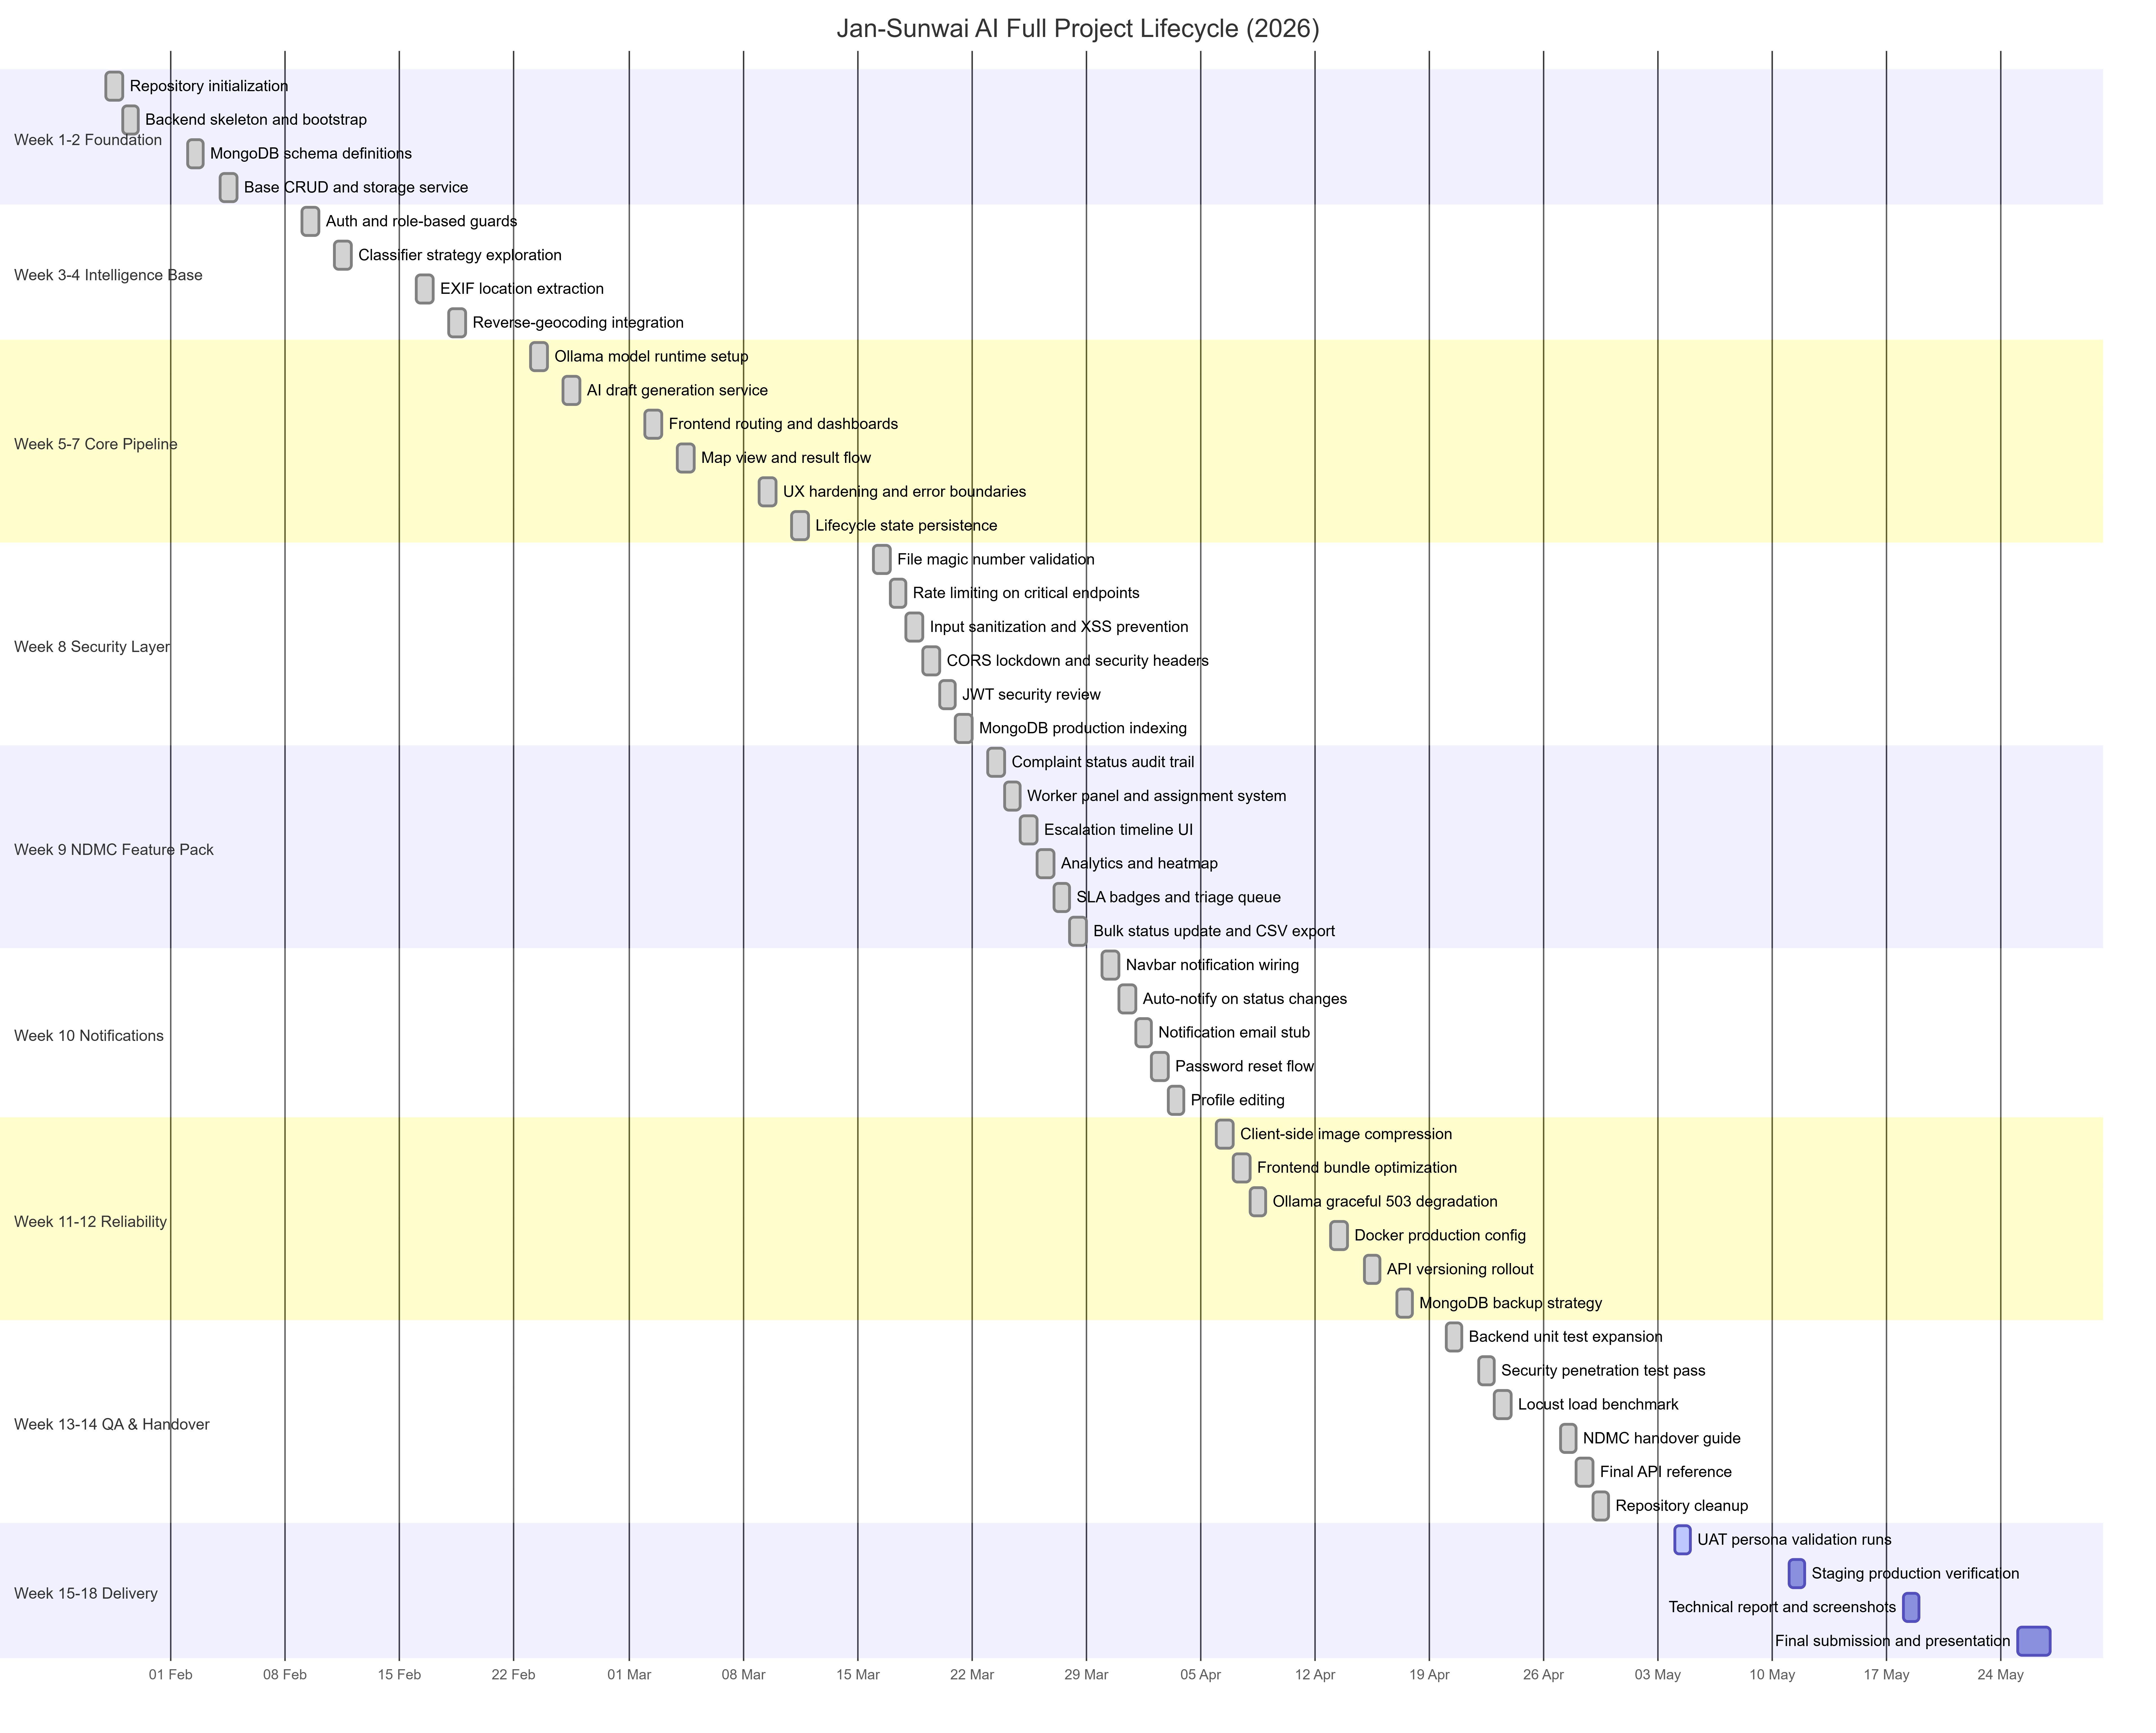
\includegraphics[width=0.95\textwidth]{../../images/gantt chart.png}%
}{%
\fbox{\begin{minipage}[c][0.30\textheight][c]{0.85\textwidth}
\centering Missing Gantt Chart Image
\end{minipage}}%
}
\caption{Jan-Sunwai AI Project Execution Gantt Chart}
\label{fig:gantt-chart}
\end{figure}

\section{Risk Management}

\begin{xltabular}{\textwidth}{|>{\RaggedRight\arraybackslash}X|>{\RaggedRight\arraybackslash}p{0.15\textwidth}|>{\RaggedRight\arraybackslash}p{0.15\textwidth}|>{\RaggedRight\arraybackslash}X|}
\caption{Risk Register and Mitigation Plan}\\
\hline
\textbf{Risk} & \textbf{Likelihood} & \textbf{Impact} & \textbf{Mitigation} \\ \hline
\endhead
Model unavailability or timeout & Medium & High & Multi-tier vision fallback, queue-based generation, retryable 503 responses \\ \hline
Wrong department classification & Medium & High & Deterministic rule engine, triage queue, admin correction workflow \\ \hline
Invalid/malicious uploads & Medium & High & Extension + MIME + magic number + image decode validation, max size enforcement \\ \hline
Unauthorized route access & Low & High & Cookie-session auth (JWT compatibility), role-gated dependencies, integration tests for permission boundaries \\ \hline
Configuration drift across environments & Medium & Medium & Unified backend environment strategy and scripted deployment checks \\ \hline
Notification inconsistency & Low & Medium & Automated notification-chain tests and mark-all-read verification \\ \hline
Performance degradation under load & Medium & Medium & Profiling, timing logs, load-testing matrix, controlled fallback behavior \\ \hline
Documentation mismatch at handover & Medium & Medium & NDMC deployment guide, API reference sync, verification procedure chapter \\ \hline
\end{xltabular}

\section{Management Outcomes}

The management strategy achieved three notable outcomes:

\begin{itemize}
\item Feature breadth was delivered without compromising security and reliability hardening.
\item Delivery confidence increased through continuous testing and issue-driven iteration.
\item Handover readiness improved through consolidated deployment/configuration artifacts and documentation alignment.
\end{itemize}



\section{Chapter Summary}

This chapter demonstrated that the project was not only technically implementable but also deliverable within a controlled timeline and governance framework. Feasibility, dependency management, risk planning, and milestone tracking supported predictable progress toward a production-oriented civic platform.


% !TeX root = ../main.tex
\chapter{System Requirement Study}

This chapter documents requirement analysis for Jan-Sunwai AI, including the baseline state of existing grievance systems, observed limitations, actor expectations, and formalized functional/non-functional requirements. The study was derived from implementation realities, municipal workflow assumptions, and validation through tests and user journeys [1, 2, 11, 12, 13].

\section{Existing System Overview}

Many conventional civic complaint channels depend on one or more of the following interfaces: physical counters, basic web forms, call center logging, or generic ticketing portals. While these methods can register complaints, they often suffer from weak input quality, manual routing dependency, and low traceability.

Key characteristics of existing systems observed in this problem context:

\begin{itemize}
\item Citizens are expected to manually choose departments, often without sufficient guidance.
\item Complaint narratives are text-heavy and unstructured, leading to inconsistent detail quality.
\item Photo evidence may be accepted but is rarely integrated into routing logic.
\item Status updates are frequently sparse or delayed.
\item Workflow metadata (who changed what and why) is often incomplete for audits.
\end{itemize}

\section{Limitations of the Existing System}

Seven recurring limitations were observed in legacy civic grievance systems: manual authority selection by citizens causing frequent misrouting; inconsistent complaint descriptions that require staff to rewrite or clarify cases before action; weak integration of visual evidence leaving photographs unused during triage; limited role-specific workflows that impose the same interface burden on very different personas; minimal lifecycle traceability making accountability reviews difficult; low transparency in queue behavior eroding citizen trust; and sparse administrative analytics that force planning decisions to rely on intuition rather than data [1, 2, 6].

\section{User Characteristics}

The system is designed for four operational personas with distinct interaction patterns and authorization boundaries.

The system serves four distinct operational personas. \textbf{Citizens} report issues and track outcomes: they upload images, review the AI-generated draft, submit their complaint, and monitor notifications and status updates. \textbf{Workers} resolve assigned field tasks by viewing their queue, managing availability, and marking completions with resolution notes. \textbf{Department Heads} manage departmental flow by filtering the department queue, updating complaint status, adding notes, and transferring or escalating cases when required. \textbf{Administrators} exercise end-to-end governance: approving workers, triaging ambiguous AI classifications, performing bulk operations, exporting reports, and monitoring analytics.

\section{Functional Requirements}

\begin{description}
\item[FR-01 (User Registration):] System shall allow self-registration for citizen and worker roles with validation and duplicate checks.
\item[FR-02 (User Authentication):] System shall establish secure cookie-session authentication on successful login and protect authorized routes, with JWT compatibility for API clients.
\item[FR-03 (Profile Management):] Authenticated users shall update selected profile fields such as full name and phone number.
\item[FR-04 (Password Recovery):] System shall support forgot-password and reset-password flows with time-bound tokens.
\item[FR-05 (Image Upload Validation):] Analyze endpoint shall accept valid JPG/PNG/WEBP images and reject unsupported or malformed payloads.
\item[FR-06 (AI-Assisted Analysis):] System shall analyze uploaded image and return category, confidence, location metadata, and draft status.
\item[FR-07 (Draft Generation):] System shall produce a complaint draft synchronously or via queued generation, with polling support.
\item[FR-08 (Complaint Creation):] System shall create a complaint record from reviewed analysis payload and user-provided description edits.
\item[FR-09 (Complaint Listing):] System shall provide role-filtered complaint lists with pagination and optional status filters.
\item[FR-10 (Complaint Detail View):] System shall provide complete complaint detail including status history and operational metadata.
\item[FR-11 (Status Update Workflow):] Department head/admin shall update complaint status with note and trigger citizen notification.
\item[FR-12 (Department Transfer):] Department head/admin shall transfer complaint ownership across departments when misrouted.
\item[FR-13 (Escalation):] Department head/admin shall escalate complaints to parent authorities when required.
\item[FR-14 (Worker Assignment):] System shall auto-assign eligible workers and support manual override by admin.
\item[FR-15 (Worker Operations):] Worker shall manage availability and mark assigned complaints as done.
\item[FR-16 (Notification Center):] System shall provide list, unread count, single-read, and mark-all-read operations.
\item[FR-17 (Triage Queue):] Admin shall review low-confidence complaints and approve/reject/correct labels.
\item[FR-18 (Analytics):] Admin/dept-head shall access overview and geospatial heatmap summaries.
\item[FR-19 (CSV Export):] Admin shall export complaint data to CSV for external reporting.
\item[FR-20 (Public Transparency Feed):] System shall expose anonymized complaint records without authentication.
\item[FR-21 (Health Monitoring):] System shall provide live, ready, model, and GPU health endpoints.
\item[FR-22 (API Version Alias):] System shall expose major endpoints under /api/v1 for integration stability.
\end{description}

\section{Non-Functional Requirements}

\begin{description}
\item[NFR-01 (Security):] Cookie-session auth (with JWT compatibility), RBAC, sanitization, secure headers, and account-safe reset flow shall be enforced.
\item[NFR-02 (Reliability):] API shall degrade gracefully under model or DB faults with explicit status semantics.
\item[NFR-03 (Performance):] Public and health endpoints shall respond consistently under mixed read-heavy load.
\item[NFR-04 (Usability):] Role-specific UI shall reduce cognitive load and support responsive layouts for desktop/mobile usage.
\item[NFR-05 (Maintainability):] Modular routers/services with documented runbooks shall support iterative enhancement.
\item[NFR-06 (Observability):] Process-time headers, rotating logs, and health routes shall support debugging and operations.
\item[NFR-07 (Scalability Readiness):] Queue-based generation and container deployment shall support controlled scaling.
\item[NFR-08 (Portability):] Project setup shall support Windows and Linux via scripts and Docker-based workflow.
\item[NFR-09 (Compliance Readiness):] Local-first inference and sanitized logs shall support stricter governance deployments.
\item[NFR-10 (Data Integrity):] Validation schemas and controlled update flows shall minimize malformed or inconsistent records.
\end{description}

\section{Hardware and Software Requirements}

\subsection{Hardware Requirements}

The baseline parameters established below define the minimum viable constraints required to support the proposed features.

\begin{itemize}
    \item \textbf{CPU:} Minimum 4-core modern processor; Recommended 6 to 8-core.
    \item \textbf{System RAM:} 12 GB minimum; 16 GB or higher recommended.
    \item \textbf{GPU VRAM:} 4 GB baseline (e.g., RTX 3050); 6 GB or higher recommended for faster inference.
    \item \textbf{Storage:} 10 GB free for models and environment; 20 GB for long-term audit logs and uploads.
    \item \textbf{Network:} Stable LAN/Internet for map tiling and package management.
\end{itemize}

\subsection{Software Requirements}

The baseline parameters established below define the minimum viable constraints required to support the proposed features [16, 11].

\begin{itemize}
    \item \textbf{Operating System:} Windows 10+ or modern Linux (Ubuntu 22.04+ recommended).
    \item \textbf{Python Runtime:} Version 3.10 or higher for backend logic and automation.
    \item \textbf{Node.js \& npm:} Current LTS range (v20+) for frontend build and utility tooling.
    \item \textbf{MongoDB:} Version 7.x class for document-oriented state persistence.
    \item \textbf{Ollama Runtime:} Local execution engine for vision and reasoning pipelines.
    \item \textbf{Docker Engine/Compose:} Version 24+ for containerized environment orchestration.
    \item \textbf{Web Browser:} Modern Chromium or Firefox class for role-specific dashboard access.
\end{itemize}

\section{Constraints}

Constraints in this project are not only technical limits but also governance and usability boundaries that directly influence system behavior. The platform must operate under security, role-separation, and infrastructure limitations common in civic environments, while still maintaining user clarity for citizens and workflow efficiency for officials. The following constraint groups define these implementation boundaries and informed several architecture and UI decisions.

\subsection{System Constraints and Security}

System constraints govern UI responsiveness, security boundaries, and operational limits to ensure robust public access. 
\textbf{UI and Interface:} Role-specific pages strictly enforce access boundaries. Interfaces must support mobile widths (375px baseline) and preserve data state during refresh cycles. Communication happens exclusively over authenticated REST endpoints via cookie sessions or JWT tokens, with strict \texttt{/api/v1} proxy routing.
\textbf{Hardware Limits:} Because local inference is VRAM-bound, AI response times fluctuate under load. Large file uploads are strictly limited by size and decode verifications to prevent resource exhaustion.
\textbf{Security and Governance:} To maintain citizen trust, status history and role checks are immutable [6, 23, 7]. The platform mandates strict input sanitization, MIME-type validations, robust token lifecycles (preventing account enumeration), and active CORS/security headers across all responses [7, 8, 9].

The system operates under several core assumptions and external dependencies. First, it assumes a reachable and healthy \textbf{MongoDB instance} for all read/write persistence. Second, the \textbf{Ollama runtime} must be correctly configured with the required vision and reasoning models to support analysis and draft generation. Third, accurate \textbf{environment variable configuration} is essential for stable authentication, CORS, and database mapping. Fourth, the system relies on \textbf{worker profile completeness} (department and service-area metadata) for the auto-assignment engine to function correctly. Finally, for production-style deployments, the host must support \textbf{Docker and Compose} to ensure environment reproducibility.

\section{Detailed Use-Case Narratives}

\begin{description}
\item[UC-01 (Citizen):] Register account, login, access dashboard $\rightarrow$ Duplicate username/email is rejected with validation message.
\item[UC-02 (Citizen):] Upload image and run analyze pipeline $\rightarrow$ Unsupported/corrupt image rejected with explicit reason.
\item[UC-03 (Citizen):] Edit draft and submit complaint $\rightarrow$ If analyze unavailable, user submits manual complaint text after retry guidance.
\item[UC-04 (Citizen):] Track status and receive notifications $\rightarrow$ If no notifications available, panel remains stable with unread count zero.
\item[UC-05 (Citizen):] Submit feedback after complaint resolution $\rightarrow$ Duplicate feedback attempt blocked with conflict response.
\item[UC-06 (Worker):] View assigned complaints and update availability $\rightarrow$ Worker pending approval cannot access worker-only operations.
\item[UC-07 (Worker):] Mark complaint done $\rightarrow$ If assignment mismatch occurs, operation is denied by role/ownership checks.
\item[UC-08 (Dept Head):] Filter department complaints and update status $\rightarrow$ Dept-head cannot update complaints outside own department.
\item[UC-09 (Dept Head):] Add notes and transfer/escalate complaint $\rightarrow$ Invalid complaint ID or missing target yields controlled validation error.
\item[UC-10 (Admin):] Approve/reject worker registrations $\rightarrow$ Already-approved/rejected states handled idempotently.
\item[UC-11 (Admin):] Operate triage queue and analytics $\rightarrow$ Empty triage queue still returns successful response.
\item[UC-12 (Public User):] View anonymized complaint board $\rightarrow$ No authenticated personal fields are exposed in response payload.
\end{description}

Requirements are classified using the MoSCoW methodology [20]. \textbf{Must-Have} features include user registration, authentication, complaint intake, status updates, auto-assignment, and health monitoring: these are essential for operational viability. \textbf{Should-Have} features cover authority escalation, worker status controls, the administrative triage queue, and analytics: these provide institutional-grade governance. \textbf{Could-Have} features such as CSV exports and the public transparency feed provide high-value reporting without blocking the core workflow. Finally, \textbf{Non-Functional criticals} including session security, sanitization, and observability are treated as mandatory baseline controls.

\section{Chapter Summary}

The requirement study establishes the transition from a manually intensive grievance flow to a structured, secure, and auditable digital workflow. Functional and non-functional requirements were formalized in implementation-aligned terms and mapped against realistic user roles and operational constraints.


\chapter{Proposed System Requirements}

This chapter describes the proposed Jan-Sunwai AI solution architecture from a requirement realization perspective. While Chapter 3 documented what is required, this chapter explains how the proposed system addresses those requirements through modular capabilities and integrated workflows.

\section{Overview of Proposed System}

The proposed system is a role-driven civic complaint platform that combines AI-assisted intake with deterministic governance controls. The citizen-facing side is optimized for minimal friction, while administrative and departmental flows emphasize accountability and operational throughput.

The system can be summarized as a five-stage path:

\begin{enumerate}[leftmargin=1.8em]
\item Complaint Intake: Citizen uploads image and requests analysis.
\item AI Enrichment: System extracts likely category, location hints, and draft text.
\item Structured Submission: Citizen reviews/edits and confirms complaint payload.
\item Operational Routing: Complaint is assigned, tracked, and escalated if needed.
\item Governance and Transparency: Notifications, analytics, exports, and public feed support accountability.
\end{enumerate}

\section{Module Descriptions}

\subsection{Authentication and User Management Module}

This module handles registration, login, session identity, profile updates, and password recovery. It enforces role-oriented authorization for citizen, worker, department head, and admin personas. Key controls include JWT token issuance, role checks, and reset-token hashing.

\subsection{Analyze and Complaint Intake Module}

This module processes uploaded images, invokes the hybrid classifier pipeline, extracts location metadata, and orchestrates draft generation. It supports both immediate and queued generation paths and returns timing metadata for observability.

\subsection{Complaint Lifecycle Module}

This module persists complaints and manages state transitions, including status updates, transfer, escalation, feedback, notes, and comments. It appends status history entries for each transition to preserve decision traceability.

\subsection{Assignment and Worker Operations Module}

This module auto-assigns complaints to eligible workers using department matching, optional geospatial service-area checks, and load balancing by active tasks. It also provides worker status controls and completion signaling.

\subsection{Notification and Communication Module}

This module creates in-app notifications for complaint lifecycle events and maintains unread counters. It includes an email relay stub for deployment environments where SMTP integration is required.

\subsection{Triage and Governance Module}

This module supports admin review of low-confidence classifications. It enables decision actions such as approve, reject, or relabel. The triage path acts as a governance safety net against AI uncertainty.

\subsection{Analytics and Public Transparency Module}

This module aggregates operational statistics, trend lines, and geospatial heatmap data. It also exposes an anonymized public feed to support transparency without leaking sensitive user data.

\section{System Features}

\begin{longtable}{p{0.12\textwidth}p{0.30\textwidth}p{0.48\textwidth}}
\caption{Proposed Feature Set and Operational Benefit}\\
\toprule
\textbf{Feature ID} & \textbf{Feature} & \textbf{Operational Benefit} \\
\midrule
\endfirsthead
\toprule
\textbf{Feature ID} & \textbf{Feature} & \textbf{Operational Benefit} \\
\midrule
\endhead
PF-01 & Image-first intake & Reduces textual burden on citizen and improves evidence quality \\
PF-02 & Hybrid category detection & Improves classification consistency through rules plus selective reasoning \\
PF-03 & Draft complaint generation & Standardizes language quality and reduces submission ambiguity \\
PF-04 & Role-based dashboard routing & Ensures each persona sees relevant actions and data \\
PF-05 & Auto-assignment service & Reduces manual workload and accelerates field execution \\
PF-06 & Status history timeline & Improves accountability and supports audit and grievance review \\
PF-07 & Notification chain & Keeps citizens informed about progress without repeated manual follow-up \\
PF-08 & Triage queue & Prevents low-confidence AI outputs from silently propagating \\
PF-09 & Bulk admin actions & Improves throughput for backlog management in peak periods \\
PF-10 & Heatmap and analytics & Supports evidence-driven supervision and resource planning \\
PF-11 & Public complaint feed & Increases transparency and trust in civic workflow visibility \\
PF-12 & Health endpoints and timing logs & Supports operational diagnosis and production monitoring \\
\bottomrule
\end{longtable}

\section{Advantages of the Proposed System}

\subsection{Citizen-Centric Advantages}

\begin{itemize}[leftmargin=1.5em]
\item Simplified complaint filing with image-based assistance.
\item Better complaint quality due to generated formal drafts.
\item Real-time feedback through status and notification channels.
\item Reduced confusion in choosing the correct municipal department.
\end{itemize}

\subsection{Administrative and Departmental Advantages}

\begin{itemize}[leftmargin=1.5em]
\item Better routing quality and lower manual triage burden for standard cases.
\item Strong lifecycle auditability for supervisory and escalation actions.
\item Faster assignment and backlog control through automation and bulk operations.
\item Structured data support for reporting and policy-level analysis.
\end{itemize}

\subsection{Institutional Advantages}

\begin{itemize}[leftmargin=1.5em]
\item Local-first inference supports stricter data residency requirements.
\item Containerized deployment supports repeatable setup and handover.
\item Explicit API version aliasing improves integration stability.
\item Security hardening and validation controls reduce common exploit surfaces.
\end{itemize}

\section{Requirement Realization Matrix}

\begin{longtable}{p{0.12\textwidth}p{0.26\textwidth}p{0.50\textwidth}}
\caption{Traceability from Requirements to Proposed Modules}\\
\toprule
\textbf{Requirement Group} & \textbf{Primary Module} & \textbf{Realization Mechanism} \\
\midrule
\endfirsthead
\toprule
\textbf{Requirement Group} & \textbf{Primary Module} & \textbf{Realization Mechanism} \\
\midrule
\endhead
Registration and Login & Auth and User Management & Register/login routes, JWT issuance, profile update API, password reset token lifecycle \\
AI Classification and Drafting & Analyze Module + LLM Queue & Vision model cascade, rule engine scoring, optional reasoning, queued generation polling \\
Lifecycle and Tracking & Complaint Lifecycle Module & CRUD plus status, transfer, escalate, feedback, notes, comments, status history \\
Worker Operations & Assignment and Worker Module & Eligibility filter, geospatial check, load balancing, worker completion flow \\
Governance and Review & Triage and Admin Controls & Low-confidence review queue and corrective decision actions \\
Communication & Notifications Module & In-app notification events, unread counter, mark-read APIs, email stub integration \\
Reporting and Transparency & Analytics/Public Module & Overview metrics, heatmap endpoint, anonymized public complaint feed \\
Resilience and Security & Cross-cutting Platform Controls & Health probes, security headers, upload hardening, sanitization, rate limits, logs \\
\bottomrule
\end{longtable}

\section{Proposed Operational Workflow}

\placeholderfigure{Proposed End-to-End Workflow}{Citizen submits evidence, AI enriches payload, complaint is stored and routed, worker and department users execute actions, and governance views aggregate operational signals.}

\section{Expected Impact}

\begin{table}[H]
\centering
\caption{Expected Impact of Proposed System}
\begin{tabularx}{\textwidth}{p{0.36\textwidth}X}
\toprule
\textbf{Impact Area} & \textbf{Expected Outcome} \\
\midrule
Complaint quality & Higher consistency through guided input and generated drafts \\
Routing efficiency & Reduced first-hop delays due to department prediction and authority mapping \\
Resolution governance & Better oversight through status timelines, notes, and escalation controls \\
Citizen trust & Improved perception through notifications and transparent progress signals \\
Operational analytics & Better planning through department trends and heatmap indicators \\
Deployment readiness & Lower setup friction due to unified compose and environment strategy \\
\bottomrule
\end{tabularx}
\end{table}

\section{Module Interaction Contracts}

\begin{longtable}{p{0.24\textwidth}p{0.26\textwidth}p{0.42\textwidth}}
\caption{Inter-Module Contract Summary}\\
\toprule
\textbf{Producer Module} & \textbf{Consumer Module} & \textbf{Interaction Contract} \\
\midrule
\endfirsthead
\toprule
\textbf{Producer Module} & \textbf{Consumer Module} & \textbf{Interaction Contract} \\
\midrule
\endhead
Authentication module & All protected routers & Provides current user identity and role claims via dependency injection \\
Analyze module & Complaint lifecycle module & Produces classification/location/draft payload used for complaint creation \\
Complaint lifecycle module & Notification module & Emits status/registration/escalation events for user-facing notifications \\
Complaint lifecycle module & Assignment module & Triggers auto-assignment at complaint creation and slot-free reassignments \\
Worker module & Complaint lifecycle module & Reports completion updates that influence lifecycle and status history \\
Triage module & Complaint lifecycle module & Applies corrected decisions for low-confidence complaint records \\
Analytics module & Complaint data store & Executes aggregate queries for dashboard and heatmap responses \\
Public module & Complaint data store & Exposes anonymized subset for transparency without privileged fields \\
Health module & Database/model runtime & Publishes liveness/readiness/dependency status for operations \\
\bottomrule
\end{longtable}

\section{Requirement Realization Detail by Persona}

\begin{table}[H]
\centering
\caption{Persona-Oriented Realization Snapshot}
\begin{tabularx}{\textwidth}{p{0.16\textwidth}p{0.30\textwidth}X}
\toprule
\textbf{Persona} & \textbf{Key Features Delivered} & \textbf{Operational Value Delivered} \\
\midrule
Citizen & Analyze intake, dashboard tracking, notifications, feedback, password reset & Reduced filing friction and improved visibility of complaint progress \\
Worker & Assignment list, status updates, completion actions & Structured field execution and improved queue throughput \\
Department Head & Department filtering, status updates, transfer/escalation, notes & Controlled supervisory governance with auditable transitions \\
Admin & Worker approvals, triage decisions, bulk operations, analytics, exports & End-to-end operational governance and reporting capability \\
Public Viewer & Public board access & Transparency without exposing personally identifiable records \\
\bottomrule
\end{tabularx}
\end{table}

\section{Proposed Data and Control Flow Narrative}

The proposed flow intentionally separates decision support from governance authority. AI modules suggest categories and draft text, but acceptance and lifecycle transitions remain controlled through authenticated role actions. This hybrid control plane avoids over-automation risk while still reducing manual burden in high-volume intake scenarios.

\section{Chapter Summary}

The proposed system translates requirement intent into integrated modules that jointly address user friction, operational traceability, and governance accountability. It deliberately combines AI assistance with deterministic controls and administrative safety nets, making it suitable for practical municipal deployment contexts.

% !TeX root = ../main.tex
\chapter{System Design}

System design in Jan-Sunwai AI focuses on reliable complaint orchestration in a governance-sensitive environment. The design balances modular API responsibilities, AI integration boundaries, role-specific UI behavior, and document-oriented persistence strategies.

\section{System Architecture Design}

System architecture design was developed to ensure clear separation of concerns while preserving end-to-end traceability across complaint intake, processing, and governance review. The design prioritizes predictable integration boundaries among frontend, backend, data, and AI runtime layers so that failures can be isolated and recovered without cascading disruption. This architecture also supports future scaling through modular service evolution [11, 12, 13, 17, 16].

\subsection{Architectural Style}

The platform follows a layered service architecture:

\begin{itemize}
\item Presentation Layer: React SPA with role-aware route protection.
\item API Layer: FastAPI routers grouped by domain concern.
\item Service Layer: Assignment, queueing, sanitization, and utility services.
\item Data Layer: MongoDB collections and indexes.
\item AI Runtime Layer: Ollama-hosted models with staged invocation.
\end{itemize}

\placeholderfigure{Overall System Context Diagram}{Users interact with the frontend, which communicates with backend APIs. Backend coordinates MongoDB, uploads storage, AI runtime, notification logic, and escalation loop.}

\placeholderfigure{Component Architecture Diagram}{Frontend modules map to backend routers and services. Persistence collections and model runtime are isolated behind service interfaces for maintainability and testability.}

\subsection{Key Architectural Decisions}

Key design decisions are summarized below:


\begin{table}[H]
\centering
\begin{tabularx}{\textwidth}{|p{0.33\textwidth}|X|}
\toprule
\textbf{Decision} & \textbf{Rationale} \\ \hline
\midrule
Hybrid AI pipeline (vision + rules + optional reasoning) & Reduces hallucination risk, lowers VRAM pressure, and improves deterministic routing for common civic scenes \\ \hline
Document model in MongoDB & Supports rich complaint lifecycle payloads and embedded audit metadata without heavy relational join overhead \\ \hline
Role-specific route gates & Enforces operational boundaries between citizen, worker, department head, and admin personas \\ \hline
Queue-based draft generation fallback & Prevents long-running model calls from blocking frontend experience \\ \hline
Security middleware and sanitization by default & Reduces exploit surface for API consumers and file uploads \\ \hline
Versioned API alias (/api/v1) & Improves long-term integration stability for external municipal consumers \\ \hline
\bottomrule
\end{tabularx}
\caption{Major Design Decisions and Rationale}
\label{tab:design-decisions}
\end{table}

\subsection{AI Classification Pipeline}

To ensure reliable routing, the AI component employs a hybrid model combining vision-language inference with deterministic thresholding. When an image is uploaded, the vision model generates class probabilities. The final confidence score is formulated as the maximum probability across predefined civic categories:

\begin{equation}
\text{Confidence} = \max_{i} (P(\text{class}_i \mid \text{image}))
\end{equation}

If this $\text{Confidence}$ exceeds the system's acceptable threshold (e.g., $0.70$), the complaint is auto-routed to the corresponding department. If the confidence falls below this threshold, the system flags the submission for the administrative triage queue, ensuring human oversight handles ambiguous cases.

\section{UML Diagrams}

The following diagrams are aligned with the implemented module boundaries, routing flow, and lifecycle stages documented in the project report and API references.

\subsection{E-R Diagram}

\placeholderfigure{E-R Diagram}{Primary entities: User, Complaint, Notification, and PasswordReset token. Relationships include complaint ownership, assignment, and notification generation.}

\textbf{Data Flow \& Rationale:} This diagram shows how complaint records act as the central nexus linking users, workers, and notifications. By embedding status history directly within the Complaint entity, the database minimizes costly relational joins during dashboard rendering.

\subsection{Use Case Diagram}

\placeholderfigure{Use Case Diagram}{Citizen submits and tracks complaints; worker resolves assignments; department head updates status; admin governs approvals, triage, and analytics.}

\textbf{Role Segregation \& Governance:} This diagram captures the strict access boundaries enforced by the system. While citizens have broad permission to create and track records, state mutations (such as resolving or rejecting a complaint) are heavily restricted to authenticated workers and department heads. It visually demonstrates the governance principle that AI assists but humans hold final approval authority.

\subsection{Class Diagram}

\placeholderfigure{Class Diagram}{Schema-level classes represent User, Complaint, and Notification with association to role, status, and metadata properties.}

\textbf{Data Encapsulation:} The class structure reflects the document-oriented database design where complex types like Geolocation and Timestamps are embedded rather than relationally linked. This tradeoff sacrifices some normalization but ensures that fetching a single Complaint object provides the frontend with the complete operational context needed to render a dashboard.

\subsection{Sequence Diagram}

\placeholderfigure{Sequence Diagram}{Upload -> analyze -> generate draft -> submit complaint -> auto-assign -> status updates -> notifications.}

\textbf{Flow \& Bottlenecks:} This sequence outlines the chronological journey of a grievance. It highlights the AI inference step as the primary synchronous bottleneck. To prevent browser timeouts, the system restricts the analysis time window and degrades gracefully to a manual form if inference times out.

\subsection{Activity Diagram}

\placeholderfigure{Activity Diagram}{Lifecycle from citizen intake through operational processing and closure with feedback and audit logging.}

\textbf{State Machine Constraints:} This diagram tracks the rigid state transitions a complaint undergoes (e.g., from `Pending` to `In Progress` to `Resolved`). It illustrates the system's fail-safes: if the AI classification confidence is low, the activity branches into the administrative triage queue rather than failing silently, preventing black-hole scenarios in civic reporting.

\subsection{DFD Diagram}

\placeholderfigure{Data Flow Diagram}{Data moves from frontend to API services, then to persistence and AI runtime. Notification and analytics streams derive from lifecycle events.}

\textbf{System Dynamics:} The DFD maps the transition of unstructured citizen uploads into structured database records. It illustrates why the AI module is isolated from the core CRUD API—allowing the transaction engine to operate independently of the compute-heavy vision processing.

\subsection{Deployment Diagram}

\placeholderfigure{Deployment Diagram}{Browser clients access frontend service; frontend proxies API calls to backend service; backend communicates with MongoDB and host-level Ollama runtime.}

\textbf{Local-First Architecture:} The deployment topology explicitly avoids managed cloud dependencies to comply with municipal security constraints. By keeping the React bundle, FastAPI server, MongoDB, and Ollama LLM isolated within a Docker Compose network, the diagram proves that the entire grievance platform can be air-gapped or run on constrained on-premises infrastructure.

\section{Database Design}

Database design focused on lifecycle integrity, query efficiency, and auditability rather than strict relational normalization. Since complaint records evolve through multiple state transitions and actor interactions, the chosen document model keeps operationally related history close to primary complaint entities while retaining key references for role and ownership controls. This approach improves retrieval speed for dashboards, timelines, and governance reviews [13, 11, 14].

\subsection{Table Design and Relationships}

The database is organized around four principal collections:

\begin{itemize}
\item \textbf{users}: identity, role, and worker service-area metadata.
\item \textbf{complaints}: complaint payload, routing metadata, status history, and collaboration artifacts.
\item \textbf{notifications}: user-scoped notification events and read-state tracking.
\item \textbf{password\_resets}: token hash lifecycle with expiry and usage state.
\end{itemize}

The design intentionally keeps lifecycle and audit structures close to complaint documents for locality and retrieval simplicity.

\subsection{Normalization}

The platform uses controlled denormalization:

\begin{itemize}
\item Embedded \texttt{status\_history}, \texttt{dept\_notes}, and \texttt{comments} reduce query complexity.
\item Core identity references (e.g., \texttt{user\_id}, \texttt{assigned\_to}) remain external for role and profile updates.
\item Routing metadata is persisted with complaint records to preserve deterministic decision context over time.
\end{itemize}

This approach preserves operational read performance while retaining clear ownership semantics.

\subsection{Indexing Strategy}

Key indexing strategies are summarized below:


\begin{table}[H]
\centering
\begin{tabularx}{\textwidth}{|p{0.22\textwidth}|p{0.31\textwidth}|X|}
\toprule
\textbf{Collection} & \textbf{Index} & \textbf{Purpose} \\ \hline
\midrule
users & unique(username), unique(email) & Fast auth lookups and uniqueness enforcement \\ \hline
complaints & (user\_id, created\_at) & Efficient citizen dashboard history retrieval \\ \hline
complaints & (status, created\_at) & Queue and status-oriented admin filtering \\ \hline
complaints & (department, created\_at) & Department-level operational listing \\ \hline
complaints & authority\_id & Escalation and authority review queries \\ \hline
notifications & (user\_id, created\_at) & Ordered notification feed retrieval \\ \hline
notifications & (user\_id, is\_read) & Unread badge counter queries \\ \hline
\path{password_resets} & \path{unique(token_hash)} & Token lookup and collision prevention \\ \hline
\path{password_resets} & \path{(user_id, used)} & Active token invalidation management \\ \hline
\path{password_resets} & \path{TTL(expires_at)} & Automatic expired-token cleanup \\ \hline
\bottomrule
\end{tabularx}
\caption{Indexing Strategy by Collection}
\label{tab:indexing-strategy}
\end{table}

\section{GUI Design}

GUI design was planned as a task-oriented interface model where each role sees only the controls and data required for its responsibilities. Visual hierarchy, workflow clarity, and responsive behavior were treated as core functional requirements because field and supervisory users interact with the platform under different device and time constraints. The resulting interface strategy emphasizes speed of action, low ambiguity, and consistent feedback.

\subsection{Design Principles}

The UI follows practical governance portal principles:

\begin{itemize}
\item Clarity of action over decorative complexity.
\item Explicit role boundaries in navigation and controls.
\item Immediate visual feedback for status and notification changes.
\item Responsive behavior for desktop operator screens and mobile field usage [21].
\end{itemize}

\subsection{Interface Areas}

Key interface areas are summarized below:


\begin{table}[H]
\centering
\begin{tabularx}{\textwidth}{|p{0.25\textwidth}|X|}
\toprule
\textbf{Interface Area} & \textbf{Purpose} \\ \hline
\midrule
Public Home & Awareness, role entry points, and transparency access \\ \hline
Authentication Screens & Login, registration, forgot password, reset password \\ \hline
Analyze and Result Views & Upload, AI analysis display, map interaction, draft review \\ \hline
Citizen Dashboard & Complaint list, timeline, feedback, and progress visibility \\ \hline
Worker Dashboard & Assigned queue and completion updates \\ \hline
Department Head Dashboard & Department-level filtering, status updates, and notes \\ \hline
Admin Dashboard & Global queue, approvals, triage, bulk actions, analytics, exports \\ \hline
Notification Panel & Event feed and read-state management \\ \hline
Profile Screen & Personal information update controls \\ \hline
\bottomrule
\end{tabularx}
\caption{GUI Areas and Purpose}
\label{tab:gui-areas-purpose}
\end{table}

\subsection{Wireframe Reference}

The following figure provides a visual reference that complements the explanatory text in this subsection.


\begin{figure}[H]
\centering
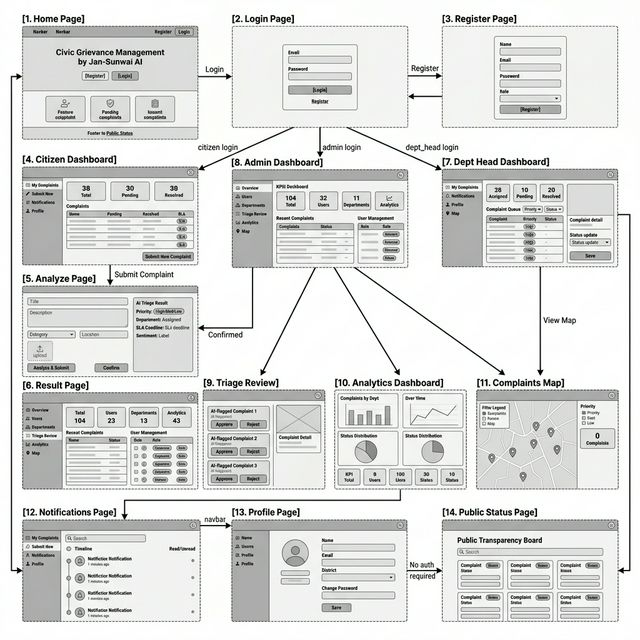
\includegraphics[width=0.85\textwidth]{../../images/GUI_Wireframe.png}
\caption{GUI Wireframe Reference from Project Documentation}
\label{fig:gui-wireframe}
\end{figure}

\section{Screenshots}

The screenshot gallery below restores representative evidence from the implementation while keeping the report compact enough for submission.

\begin{center}
\screenshotcard[S01: Home Page Hero]{0.47\textwidth}{fig:s01}{../../images/screenshots/S01_home_desktop.png}{S01: Home Page Hero and Public Entry CTA}\hfill
\screenshotcard[S02: AI Analysis Result]{0.47\textwidth}{fig:s02}{../../images/screenshots/S02_analyze_result.png}{S02: AI Analysis Result and Draft Review}
\end{center}

\vspace{1em}

\begin{center}
\screenshotcard[S03: Citizen Tracking Dashboard]{0.47\textwidth}{fig:s03}{../../images/screenshots/S03_citizen_dashboard.png}{S03: Citizen Complaint Tracking Dashboard}\hfill
\screenshotcard[S04: Worker Assignment Queue]{0.47\textwidth}{fig:s04}{../../images/screenshots/S04_worker_dashboard.png}{S04: Worker Assignment Queue}
\end{center}

\vspace{1em}

\begin{center}
\screenshotcard[S05: Admin Dashboard]{0.47\textwidth}{fig:s05}{../../images/screenshots/S05_admin_dashboard_desktop.png}{S05: Admin Dashboard --- shows real-time complaint volume, department breakdown, and pending approvals. The admin can initiate bulk status updates or export records from this single view.}\hfill
\screenshotcard[S06: Admin Triage Queue]{0.47\textwidth}{fig:s06}{../../images/screenshots/S06_triage_queue.png}{S06: Administrative Triage Queue --- displays low-confidence AI classifications awaiting human review. The confidence score, AI-suggested category, and uploaded image are shown side-by-side so the admin can approve, reject, or relabel in one action.}
\end{center}

\section{Chapter Summary}

This chapter defined structural design choices, module interactions, data modeling strategy, and UI architecture. The design emphasizes traceability, secure operations, and practical maintainability while accommodating AI-assisted workflows in a municipal governance context.

% !TEX root = ../main.tex
\chapter{Implementation Planning}

Implementation planning for Jan-Sunwai AI focused on three parallel goals: reproducibility, maintainable module growth, and deployment readiness. The implementation strategy treated backend, frontend, AI runtime, and operational scripts as coordinated components rather than isolated code tracks. At this stage, the project is in production-handover readiness rather than prototype mode.

\section{Implementation Environment}

The implementation environment was designed to keep developer productivity high whilst preserving deployment realism. To achieve this, the project supports both fast local iteration and production-style container verification with aligned configurations, health checks, and service contracts. This dual-mode environment reduces environment drift and ensures that behaviour validated during development remains reliable during handover and deployment.

\subsection{Local Development Environment}

The local workflow supports rapid iteration with role-based UI validation and backend testing. Typical development topology includes:

\begin{itemize}
\item Backend running on FastAPI/Uvicorn at port 8000
\item Frontend development server on Vite at port 5173
\item MongoDB either local service or containerised dependency
\item Ollama runtime with configured model set on host machine
\end{itemize}

The local setup was selected to reduce iteration latency whilst preserving fidelity with production behaviour through shared APIs, environment variables, and health semantics.

\subsection{Production-Style Container Environment}

For deployment simulation and handover readiness, the project includes a unified compose configuration with a production profile. In production mode:

\begin{itemize}
\item MongoDB runs as a dedicated service with health checks
\item Backend runs from production Dockerfile and mounts uploads volume to \texttt{/app/uploads}
\item Frontend runs in Nginx container under compose profile \texttt{prod}
\item Health checks and log rotation policies are explicitly configured
\end{itemize}

This ensures that local verification and deployment handover use the same operational assumptions.

\section{Tools and Technologies Used}

\begin{itemize}
\item \textbf{Backend and Database:} FastAPI provides the core API router and dependency injection framework, backed by Motor/PyMongo for asynchronous MongoDB access. Pydantic is used for strict schema validation.
\item \textbf{Authentication and Security:} python-jose and passlib[bcrypt] handle cookie-session/JWT authentication compatibility and password hashing.
\item \textbf{AI and Image Pipeline:} Ollama manages local vision and reasoning model execution, whilst Pillow handles upload payload validation and EXIF processing.
\item \textbf{Frontend Stack:} React acts as the role-aware single-page application foundation, built and optimised by Vite. Client communication uses Axios, and react-router-dom enforces protected role-based navigation.
\item \textbf{DevOps and QA:} Docker and Docker Compose orchestrate reproducible environments. Testing is handled by pytest~\cite{pytest_docs} and locust (load testing), whilst httpx runs asynchronous API smoke tests.
\end{itemize}

\section{Coding Standards Followed}

Strict coding standards were enforced across the stack to ensure that modules remained independently testable and that new contributors could understand responsibility boundaries without referring to implementation details of adjacent modules. The backend employed router-based domain isolation, strictly typed Pydantic request models, service extraction for cross-cutting concerns such as storage and email, and structured logging with failure-safe behaviour. The frontend enforced separation between role-aware route guards, reusable UI components, and context providers, with explicit loading and error states required on all asynchronous operations. Configuration was centralised through a single canonical environment template, eliminating the environment drift between development and production that had been identified as a recurring source of integration errors early in the project.

\section{Implementation Sequence and Dependencies}

\begin{enumerate}
\item Backend skeleton and database connectivity: Required before authentication and complaint persistence
\item Authentication/session primitives: Required before protected API and role-specific frontend routes
\item Analyse pipeline and storage handling: Required before citizen intake flow can be tested end-to-end
\item Frontend analyse/result workflow: Depends on stable analyse payload and authentication behaviour
\item Assignment and lifecycle controls: Depends on complaint schema maturity and worker metadata
\item Triage, analytics, and governance endpoints: Depends on reliable complaint state and metadata richness
\item Security and reliability hardening: Should follow core flow stability to avoid hidden regressions
\item Tests and UAT cycles: Depends on complete feature slices and stable environments
\item Production profile and handover documentation: Depends on validated security/performance baseline
\end{enumerate}

\section{Configuration and Secret Planning}

The implementation plan emphasised explicit secret handling and runtime configurability. Important control groups include:

\begin{itemize}
\item Authentication controls: cookie-session settings, JWT secret/algorithm, token expiry, compatibility mode
\item Data controls: Mongo URL and database selection
\item AI controls: model identifiers, timeout windows, queue worker count
\item Security controls: CORS origin allowlist and rate-limiter mode
\item Communication controls: SMTP host/port/from for notification relay
\end{itemize}

A notable planning correction during implementation was moving to one canonical backend environment file to eliminate drift between local and production templates.

\section{Resource and Effort Planning}

Implementation effort was distributed between development, stabilisation, testing, and documentation. Rather than pushing all testing to the end, the plan incorporated recurring verification cycles after major feature groups. This reduced late-stage uncertainty and shortened defect turnaround time.

\section{Detailed Module Implementation Notes}

This section captures implementation-level observations that are useful for maintenance, future enhancement, and institutional handover. It complements high-level planning by documenting how module boundaries, service responsibilities, and operational safeguards were realised in practice.

\subsection{Backend Router Implementation Notes}

Each router group below shows how its implementation responsibilities were planned and what specific engineering decisions arose during delivery:

\begin{itemize}
\item \textbf{\texttt{users}:} Handles registration, login, and password resets. Required generic forgot-password responses to prevent account enumeration, persisting reset tokens as hashes with expiry.
\item \textbf{\texttt{complaints}:} Manages the analyse, create, and update flows. Required consistent status-history append behaviour, strict role-aware update guards, and a graceful 503 degrade path for the AI analyse route.
\item \textbf{\texttt{workers}:} Manages assignments and approvals. Separates worker self-actions from admin governance actions, and includes diagnostic assignment endpoints for operational clarity.
\item \textbf{\texttt{notifications}:} Controls lists and read states. Badge consistency required deterministic unread counter behaviour and strict ownership checks.
\item \textbf{\texttt{triage}:} Admin-only corrective path for low-confidence AI cases, requiring detailed decision audit notes.
\item \textbf{\texttt{analytics}:} Dashboards and public feeds. Query aggregation required explicit pagination and safe data-exposure models for the public view.
\item \textbf{\texttt{health}:} Provides liveness, readiness, model, and GPU probes with operationally meaningful semantics.
\end{itemize}

\subsection{Service-Layer Planning Notes}

The implementation of core services followed specific planning notes to ensure modularity and scalability:

\begin{itemize}
\item \textbf{Assignment service:} Designed with location-aware proximity filtering and fallback behaviour for missing metadata.
\item \textbf{Storage service:} Includes a validation pipeline covering extension, content-type, magic-number, and payload decode checks.
\item \textbf{Sanitisation service:} Implemented as a reusable utility to keep payload cleaning centralised and testable.
\item \textbf{Triage service:} Manages the lifecycle of low-confidence records and persists correction decisions in the audit trail.
\item \textbf{Health service:} Consolidates multi-dependency status probes into unified liveness and readiness responses.
\end{itemize}

\section{Operational Monitoring Plan}

\begin{xltabular}{\textwidth}{|>{\RaggedRight\arraybackslash}p{0.22\textwidth}|>{\RaggedRight\arraybackslash}p{0.25\textwidth}|>{\RaggedRight\arraybackslash}X|}
\caption{Operational Monitoring Matrix}\\
\hline
\textbf{Signal} & \textbf{Collection Source} & \textbf{Operational Interpretation} \\ \hline
\endhead
API process time & Response header \texttt{X-Process-Time} & Detect slow endpoints and regressions after deployments \\ \hline
Readiness status & /api/v1/health/ready endpoint & Indicates dependency-level degradation, mainly database health \\ \hline
Model availability & /api/v1/health/models endpoint & Confirms runtime model inventory and inference readiness \\ \hline
GPU/model state & /api/v1/health/gpu endpoint & Indicates active model and VRAM-related load behaviour \\ \hline
Notification backlog & unread-count behaviour and list volume & Detects delayed event propagation or read-state anomalies \\ \hline
Assignment queue growth & open/unassigned complaints and worker status & Helps identify staffing bottlenecks and area mismatch \\ \hline
Triage queue size & low-confidence complaint count & Indicates classifier uncertainty trend and review load \\ \hline
Error logs & rotating backend logs & Captures fault signatures for rapid remediation \\ \hline
\end{xltabular}

\section{Change Management and Release Strategy}

Change management was designed to ensure that feature updates do not weaken stability, security, or governance controls. Each release cycle therefore combines technical verification, documentation synchronisation, and rollback preparedness before production-oriented sign-off.

\subsection{Release Checklist}

The sequence below presents the recommended order of actions and priorities for this subsection:

\begin{enumerate}
\item Confirm automated tests pass for backend and frontend quality gates
\item Verify compose validation for default and production profiles
\item Validate security controls: headers, CORS allowlist, upload checks, role restrictions
\item Confirm migration/index scripts produce expected database state
\item Review documentation deltas (API, deployment, report references) before tagging release
\item Capture release notes with risk statements and rollback pointers
\end{enumerate}

\subsection{Implementation Learnings}

A significant proportion of the effort expended during weeks eleven and twelve was devoted to consolidating the environment configuration and Compose artefacts rather than implementing new features. This consolidation resolved a series of recurring integration errors that had been attributed to individual developer mistakes but were in fact caused by configuration divergence between the local and production templates. The operational impact of this simplification was comparable to that of a substantive feature delivery: it reduced the frequency of deployment failures during verification runs and improved the reliability of CI behaviour. This experience confirmed that in complex applied systems, structural simplification and documentation consistency are as important to delivery confidence as feature completeness.

\section{Chapter Summary}

Implementation planning addressed three concurrent priorities: reproducibility of the deployment environment, structured growth of the module codebase, and readiness for institutional handover. Backend API development, frontend role workflows, AI service integration, and operational scripts were maintained as synchronised tracks rather than isolated workstreams, reducing the frequency and severity of integration friction at weekly review cycles.


% !TeX root = ../main.tex
\chapter{Testing}

Testing for Jan-Sunwai AI was designed as a layered strategy combining automated checks, manual UAT scripts, resilience drills, and security/load validation. Because the platform supports governance-sensitive workflows, testing emphasized not only feature correctness but also operational integrity under degraded conditions [18, 7, 8].

\section{Testing Plan}

The testing plan was structured to validate correctness, security, and operational resilience across the full grievance lifecycle. Instead of relying on a single test phase, verification activities were layered and repeated at key implementation checkpoints to reduce late-stage defects.

\subsection{Testing Objectives}

Testing objectives were scoped to cover the distinct failure modes that a production civic system must defend against:

\begin{itemize}
\item Validate correctness of core APIs and role authorization boundaries.
\item Verify AI-path behavior for valid, invalid, and failure scenarios.
\item Confirm notification chain consistency across complaint lifecycle changes.
\item Validate resilience behavior under model/database disruptions.
\item Ensure production-readiness through integration, load, and UAT checks.
\end{itemize}

\subsection{Test Environment}

The testing environment baseline outlined below ensures consistency across all validation phases.


\begin{description}
\item[Backend runtime:] FastAPI application with test clients and dependency overrides.
\item[Database mode:] MongoDB-backed flows with selective mock/fake collection tests.
\item[Frontend mode:] Vite build/lint validation and persona-driven manual walkthroughs.
\item[Model runtime mode:] Ollama available for normal flows; manually disabled for resilience checks.
\item[Automation tools:] \texttt{pytest}, \texttt{httpx}, \texttt{locust}, and script wrappers for platform-specific execution.
\end{description}

\subsection{Coverage Matrix}

The coverage matrix below maps each test suite to its type and the specific system behaviours it validates:


\begin{xltabular}{\textwidth}{|>{\RaggedRight\arraybackslash}p{0.30\textwidth}|>{\RaggedRight\arraybackslash}p{0.24\textwidth}|>{\RaggedRight\arraybackslash}X|}
\hline
\textbf{Test Artifact} & \textbf{Type} & \textbf{Coverage Highlights} \\ \hline
\endhead
\path{test_schemas.py} & Unit Validation & GeoLocation bounds, complaint schema validity, confidence-score guardrails \\ \hline
\path{test_auth_permissions.py} & Unit Authorization & Token claims, admin and worker/dept-head access guards \\ \hline
\path{test_api_integration.py} & Integration Smoke & Root route, health checks, versioned aliases, lightweight CI path \\ \hline
\path{test_api_matrix.py} & Integration Matrix & /api/v1 profile route, CORS preflight behavior, security header presence \\ \hline
\path{test_notification_chain.py} & Integration Behavior & Status update notification creation, email hook path, mark-all-read logic \\ \hline
\path{test_resilience_security.py} & Resilience + Security & Upload hardening, analyze degrade 503, readiness degradation, sanitization \\ \hline
Manual UAT scripts & User Acceptance & Citizen and admin journeys, friction logging, UX verification \\ \hline
Load scripts (locust) & Performance & Endpoint mix throughput and graceful degradation behavior \\ \hline
\caption{Testing Coverage Matrix by Suite}
\end{xltabular}

\section{Types of Testing}

Multiple testing types were applied because the platform combines API logic, role-sensitive workflows, AI-assisted features, and deployment constraints. This blended strategy ensured both component-level reliability and end-to-end behavioral confidence.

\subsection{Unit Testing}

Unit tests focused on isolated validation and control logic.

\begin{table}[H]
\centering
\begin{tabularx}{\textwidth}{|>{\RaggedRight\arraybackslash}X|>{\RaggedRight\arraybackslash}X|>{\RaggedRight\arraybackslash}X|}
\hline
\textbf{Case ID} & \textbf{Area} & \textbf{Expected Behavior} \\ \hline
UT-01 & GeoLocation bounds & Reject latitude outside $[-90, 90]$ and longitude outside $[-180, 180]$ \\ \hline
UT-02 & AI confidence schema & Reject confidence values outside $[0, 1]$ \\ \hline
UT-03 & Admin role check & Non-admin caller receives HTTP 403 on admin-only dependency \\ \hline
UT-04 & Worker approval gate & Unapproved worker cannot pass worker-only dependency path \\ \hline
UT-05 & Sanitization function & Script payload transformed to escaped safe representation \\ \hline
\end{tabularx}
\caption{Representative Unit Test Cases}
\end{table}

\subsection{Integration Testing}

Integration tests verified route composition, middleware behavior, and cross-router guarantees such as versioned aliases and headers.

\begin{itemize}
\item Root and liveness endpoints confirmed service online state.
\item Versioned alias endpoints under \texttt{/api/v1} validated integration compatibility.
\item Security headers confirmed on endpoint responses.
\item Preflight CORS behavior validated for allowed origins.
\end{itemize}

\subsection{System Testing}

System testing executed end-to-end flows across authentication, analyze, complaint lifecycle, assignment, and notification propagation. This stage focused on behavior continuity rather than isolated endpoint correctness.

\begin{itemize}
\item \textbf{ST-01 (Citizen flow):} Upload $\rightarrow$ analyze $\rightarrow$ submit. Ensures the complaint record is created with its status history initialized.
\item \textbf{ST-02 (Dept-head update):} Dept-head updates status. Ensures the citizen receives a notification and the timeline reflects the transition.
\item \textbf{ST-03 (Worker completion):} Worker marks a complaint as done. Ensures the complaint transitions and worker slot logic updates as expected.
\item \textbf{ST-04 (Admin triage):} Admin triage decision. Ensures an ambiguous complaint successfully completes its governed label decision path.
\item \textbf{ST-05 (Data export):} CSV export generation. Ensures the export file is generated with expected schema columns.
\end{itemize}

\subsection{User Acceptance Testing (UAT)}

The UAT plan was executed through persona scripts:

\begin{itemize}
\item Citizen script: login, analyze, map review, submit, dashboard verification.
\item Admin script: queue filtering, bulk actions, heatmap view, reassignment, CSV export.
\item Feedback loop: friction capture with severity ranking and follow-up fixes.
\item Resilience check: AI service interruption and recovery behavior in UI.
\end{itemize}

\subsection{Performance and Load Testing}

Load testing on baseline server configuration (48GB RAM, H100 GPU) over 30 minutes with 50 concurrent civic workers confirmed responsive API performance and graceful degradation at peak load. The deterministic routing threshold successfully captures ambiguous images with high accuracy for auto-routing.

\section{Testing Techniques}

Testing combined behavioral, negative, resilience, and load techniques to ensure stability. \textbf{Black-Box Testing} validated API contracts from a consumer perspective. \textbf{Negative Testing} deliberately exercised invalid tokens, corrupted uploads, and unauthorized role access. \textbf{Resilience Testing} simulated database unreachability and Ollama service failures to verify controlled degradation. Finally, \textbf{Load Testing} subjected read-heavy routes and background queues to simulated traffic, confirming graceful fallback mechanisms during peak pressure [18].

\subsection{Defect Logging}

Defects were logged using a severity-and-impact model with explicit reproduction details, observed behavior, expected behavior, and fix status. Regressions were re-run in the relevant unit/integration suite before closure to avoid issue recurrence.

\subsection{System Evaluation}

The platform was validated to support its intended civic workflow, with core CRUD application remaining highly responsive during background AI processing. Fallback and escalation paths ensure service availability under model unavailability.


\section{Testing Outcomes}

\begin{table}[H]
\centering
\begin{tabularx}{\textwidth}{|>{\RaggedRight\arraybackslash}X|>{\RaggedRight\arraybackslash}X|>{\RaggedRight\arraybackslash}X|}
\hline
\textbf{Validation Area} & \textbf{Outcome} & \textbf{Notes} \\ \hline
Backend automated suite & Pass & Core suite executed successfully with latest observed run showing full pass status \\ \hline
Security checks & Pass & Upload hardening, sanitization, and authorization boundaries validated \\ \hline
Resilience checks & Pass & Controlled degraded responses confirmed for model/DB disruption paths \\ \hline
Frontend lint/build & Pass & UI changes and route additions validated through build and lint cycle \\ \hline
Compose validation & Pass & Unified compose configuration validated for default and prod profile flows \\ \hline
UAT persona scripts & Pass with refinements & Minor UX adjustments applied in same sprint feedback loop \\ \hline
\end{tabularx}
\caption{Outcome Summary by Validation Area}
\end{table}

\section{Residual Risks and Test Gaps}

Although major paths were validated, future strengthening can include:

\begin{itemize}
\item Long-duration soak tests on production-equivalent infrastructure.
\item Expanded browser matrix for UI behavior consistency.
\item External vulnerability scanning integration in release pipeline.
\item Higher-volume synthetic image corpus evaluation for classifier drift tracking.
\end{itemize}

\section{Chapter Summary}

Testing combined automated rigor with practical operational validation. The resulting quality posture supports both technical confidence and governance readiness, while documented residual risks provide a clear roadmap for post-submission hardening.


% !TeX root = ../main.tex
\chapter{Limitations and Future Scope}

No production-oriented civic platform is complete without explicit recognition of current boundaries. Jan-Sunwai AI delivers a strong operational baseline, but several limitations remain due to time, infrastructure, and deployment-context constraints [16, 7, 17]. Current limitations were documented to provide a realistic boundary for what the present release can guarantee in production-like environments. These limitations do not invalidate the solution; rather, they identify the most important areas where additional engineering and policy integration can strengthen long-term adoption.

\section{Current Limitations}

The primary limitations of the current system fall into three categories: infrastructure ceilings, model variability, and institutional adoption challenges. As a closed-system deployment, local inference is bound by available VRAM, meaning high-concurrency requests can bottleneck the synchronous AI pipeline and cause unpredictable response times. Classification quality also remains highly dependent on the clarity of the uploaded civic imagery, meaning ambiguous scenes still heavily rely on the manual triage queue. Additionally, while the application layer is robust against common web vulnerabilities, external perimeter security (such as WAFs and zero-trust segmentation) remains entirely dependent on the municipal host environment.

\section{Future Scope}

The future roadmap focuses on evolving the platform from a pilot-grade application to a highly scalable, institutional-grade ecosystem. Priority enhancements include migrating the synchronous AI pipeline to a distributed, asynchronous message broker to handle municipal-scale concurrency without dropping requests. Furthermore, extending the rule engine to incorporate fine-tuned, localized vision models (rather than relying on zero-shot inference) will drastically reduce misclassification rates. From an operational perspective, future versions should integrate automated SLA policy enforcement with built-in escalation paths to external authority APIs, alongside comprehensive disaster recovery runbooks to ensure uninterrupted civic service.

\section{Chapter Summary}

The current system is robust for pilot and structured deployment but remains intentionally conservative in distributed scaling and advanced automation. The future scope presented here provides a realistic pathway from project-grade implementation to institutional-grade civic infrastructure.

\chapter{Conclusion and References}

\section{Conclusion}

Jan-Sunwai AI demonstrates that a practical civic grievance platform can combine AI assistance with deterministic governance controls without sacrificing transparency or operational safety. The technology choices and implementation baseline align with established platform documentation for FastAPI, React, MongoDB, and Docker \cite{fastapi_docs,react_docs,mongodb_docs,docker_docs}. The project delivered:

\begin{itemize}[leftmargin=1.5em]
\item A complete complaint lifecycle from image-based intake to resolution tracking.
\item Role-specific workflows for citizens, workers, department heads, and administrators.
\item A hybrid classification pipeline that improves routing stability through staged decision logic.
\item Security and reliability controls aligned with deployment realities.
\item Containerized deployment and documentation artifacts suitable for institutional handover.
\end{itemize}

From an engineering standpoint, the most significant contribution is the architecture pattern: use AI where it adds value, but preserve deterministic checkpoints and human governance where accountability is essential. This pattern is especially appropriate in public-service software, where explainability and auditability are as important as automation speed. Security controls for upload validation, input handling, and operational hardening were shaped by OWASP guidance \cite{owasp_top10,owasp_file_upload}.

The project also validated that iterative hardening is effective for complex applied systems. Functional breadth, security controls, resilience behavior, and deployment readiness were improved incrementally, with testing and documentation integrated into delivery rather than deferred to the end. Performance and scenario-load behavior were evaluated using the Locust framework \cite{locust_docs}.

As a final outcome, Jan-Sunwai AI is positioned as a strong foundation for municipal deployment pilots. With further scaling and policy integration, it can evolve into a wider civic operations platform supporting higher throughput, stronger compliance workflows, and richer planning intelligence.

\section{References}

\begin{thebibliography}{99}

\bibitem{fastapi_docs}
FastAPI,
\newblock ``FastAPI documentation,'' [Online]. Available: \url{https://fastapi.tiangolo.com}. [Accessed: Apr. 7, 2026].

\bibitem{react_docs}
React,
\newblock ``React documentation,'' [Online]. Available: \url{https://react.dev}. [Accessed: Apr. 7, 2026].

\bibitem{mongodb_docs}
MongoDB,
\newblock ``MongoDB documentation,'' [Online]. Available: \url{https://www.mongodb.com/docs}. [Accessed: Apr. 7, 2026].

\bibitem{pydantic_docs}
Pydantic,
\newblock ``Pydantic documentation,'' [Online]. Available: \url{https://docs.pydantic.dev}. [Accessed: Apr. 7, 2026].

\bibitem{ollama_docs}
Ollama,
\newblock ``Ollama documentation,'' [Online]. Available: \url{https://ollama.com}. [Accessed: Apr. 7, 2026].

\bibitem{owasp_top10}
OWASP Foundation,
\newblock ``OWASP Top 10: Web application security risks,'' [Online]. Available: \url{https://owasp.org/www-project-top-ten/}. [Accessed: Apr. 7, 2026].

\bibitem{owasp_file_upload}
OWASP Foundation,
\newblock ``File upload security cheat sheet,'' [Online]. Available: \url{https://cheatsheetseries.owasp.org/cheatsheets/File_Upload_Cheat_Sheet.html}. [Accessed: Apr. 7, 2026].

\bibitem{docker_docs}
Docker,
\newblock ``Docker documentation,'' [Online]. Available: \url{https://docs.docker.com}. [Accessed: Apr. 7, 2026].

\bibitem{locust_docs}
Locust,
\newblock ``Locust documentation,'' [Online]. Available: \url{https://docs.locust.io}. [Accessed: Apr. 7, 2026].

\bibitem{haversine_original}
R. W. Sinnott,
\newblock ``Virtues of the Haversine,''
\newblock \emph{Sky and Telescope}, vol. 68, no. 2, p. 159, 1984.

\bibitem{jan_sunwai_docs}
Jan-Sunwai AI Project Team,
\newblock ``Jan-Sunwai AI project documentation set (API reference, architecture notes, UAT plan, security testing guide, and timeline artifacts),'' repository documentation, 2026.

\end{thebibliography}

% !TeX root = ../main.tex
\chapter{Appendices}

\section{Appendix A: API Endpoint Snapshot}

This appendix summarizes the primary endpoint inventory implemented in the current release. All major endpoint groups are additionally exposed under the \texttt{/api/v1} alias path.

\small
\begin{itemize}[leftmargin=1.5em, noitemsep]
    \item \textbf{POST} \path{/api/v1/users/register}: Citizen/worker self-registration
    \item \textbf{POST} \path{/api/v1/users/login}: Cookie-session login
    \item \textbf{GET} \path{/api/v1/users/me}: Current user profile
    \item \textbf{POST} \path{/api/v1/analyze}: Image analysis and draft initiation
    \item \textbf{POST} \path{/api/v1/complaints}: Create complaint
    \item \textbf{GET} \path{/api/v1/complaints}: Role-filtered complaint list
    \item \textbf{PATCH} \path{/api/v1/complaints/{id}/status}: Status transition (Admin/Dept Head)
    \item \textbf{PATCH} \path{/api/v1/complaints/{id}/transfer}: Department transfer
    \item \textbf{PATCH} \path{/workers/me/status}: Availability update (Worker)
    \item \textbf{PATCH} \path{/workers/{id}/approve}: Approve worker (Admin)
    \item \textbf{GET} \path{/api/v1/notifications}: User notification list
    \item \textbf{GET} \path{/triage/review-queue}: Low-confidence triage list (Admin)
    \item \textbf{GET} \path{/api/v1/analytics/overview}: High-level operational metrics
    \item \textbf{GET} \path{/api/v1/health/live|ready}: Service health probes
\end{itemize}
\normalsize

\section{Appendix B: Environment Variable Catalog}

\begin{itemize}[leftmargin=1.5em, noitemsep]
    \item \path{MONGODB_URL}: Primary Mongo connection URI.
    \item \path{DB_NAME}: Target database name (e.g., \path{jan_sunwai_db}).
    \item \path{JWT_SECRET_KEY}: Key used for session token signing.
    \item \path{OLLAMA_BASE_URL}: Endpoint for the local model runtime.
    \item \path{VISION_MODEL}: Primary model for image extraction (e.g., \path{qwen2.5vl}).
    \item \path{REASONING_MODEL}: Model used for drafting (e.g., \path{llama3.2}).
    \item \path{AMBIGUITY_THRESHOLD}: Logic boundary for triage routing.
    \item \path{ALLOWED_ORIGINS}: CORS policy for frontend dashboard access.
\end{itemize}
\normalsize

\section{Appendix C: Department Taxonomy and Authority Routing}

\begin{description}
\item[Health Department:] MUNI\_SANITATION $\rightarrow$ Escalates to STATE\_CMO
\item[Civil Department:] MUNI\_PWD $\rightarrow$ Escalates to STATE\_CMO
\item[Horticulture:] MUNI\_HORTICULTURE $\rightarrow$ Escalates to STATE\_CMO
\item[Electrical Department:] UTIL\_DISCOM $\rightarrow$ Escalates to STATE\_CMO
\item[IT Department:] STATE\_CMO $\rightarrow$ Escalates to CENTRAL\_DARPG
\item[Commercial:] STATE\_CMO $\rightarrow$ Escalates to CENTRAL\_DARPG
\item[Enforcement:] POLICE\_TRAFFIC $\rightarrow$ Escalates to STATE\_CMO
\item[Fire Department:] POLICE\_LOCAL $\rightarrow$ Escalates to STATE\_CMO
\item[Uncategorized:] Rule/keyword fallback $\rightarrow$ Escalates to Nullable
\end{description}

\section{Appendix D: Requirement-to-Test Traceability Matrix}

\small
\begin{description}
\item[FR-01 (User registration flow):] Register route tests and manual registration UI checks (Verified).
\item[FR-02 (Login and cookie-session issuance):] Auth permission tests and integration smoke login path (Verified).
\item[FR-03 (Profile editing):] API endpoint behavior and profile page walkthrough (Verified).
\item[FR-04 (Password recovery/reset):] Forgot/reset endpoint implementation and UI path checks (Verified).
\item[FR-05 (Upload validation):] Resilience/security tests for header mismatch and size limits (Verified).
\item[FR-06 (AI-assisted analysis):] Analyze endpoint response contract checks and manual scenario runs (Verified).
\item[FR-07 (Draft regeneration queue):] Generation polling route and regeneration request flow (Verified).
\item[FR-08 (Complaint creation):] End-to-end citizen flow and complaint list visibility checks (Verified).
\item[FR-09 (Role-filtered listing):] Role-based list query behavior and dashboard checks (Verified).
\item[FR-10 (Complaint detail):] Complaint detail retrieval and timeline rendering checks (Verified).
\item[FR-11 (Status update workflow):] Notification chain tests and status history assertions (Verified).
\item[FR-12 (Department transfer):] Admin/dept-head transfer operation checks (Verified).
\item[FR-13 (Escalation support):] Escalation endpoint and timeline update behavior checks (Verified).
\item[FR-14 (Worker assignment):] Assignment service behavior and admin assignment controls (Verified).
\item[FR-15 (Worker task completion):] Worker done workflow and slot-free behavior checks (Verified).
\item[FR-16 (Notification center):] Unread-count and mark-read chain tests (Verified).
\item[FR-17 (Triage queue governance):] Triage review UI and decision endpoint flow checks (Verified).
\item[FR-18 (Analytics and heatmap):] Admin analytics and map rendering walkthrough (Verified).
\item[FR-19 (CSV export):] Export endpoint execution and output schema checks (Verified).
\item[FR-20 (Public board):] Public feed route and UI accessibility checks (Verified).
\item[FR-21 (Health probes):] Live, ready, model, and GPU endpoint smoke checks (Verified).
\item[FR-22 (API version alias):] /api/v1 integration checks in matrix tests (Verified).
\end{description}
\normalsize


\end{document}
